\documentclass[11pt]{article}
\renewcommand{\baselinestretch}{1.05}

\usepackage{amsmath,amsthm,verbatim,amssymb,amsfonts,amscd, graphicx}
\usepackage{graphics}

\usepackage{xcolor}

\usepackage[hidelinks]{hyperref}
\usepackage{parskip}

\usepackage{subcaption}
\usepackage{wrapfig}

% Code specific

\usepackage{listings}

\definecolor{mygreen}{rgb}{0,0.6,0}
\definecolor{mygray}{rgb}{0.5,0.5,0.5}
\definecolor{mymauve}{rgb}{0.58,0,0.82}

\lstset{ %
  backgroundcolor=\color{white},   % choose the background color; you must add \usepackage{color} or \usepackage{xcolor}
  basicstyle=\footnotesize,        % the size of the fonts that are used for the code
  breakatwhitespace=false,         % sets if automatic breaks should only happen at whitespace
  breaklines=true,                 % sets automatic line breaking
  captionpos=b,                    % sets the caption-position to bottom
  commentstyle=\color{mygreen},    % comment style
  deletekeywords={...},            % if you want to delete keywords from the given language
  escapeinside={\%*}{*)},          % if you want to add LaTeX within your code
  extendedchars=true,              % lets you use non-ASCII characters; for 8-bits encodings only, does not work with UTF-8
  frame=single,	                   % adds a frame around the code
  keepspaces=true,                 % keeps spaces in text, useful for keeping indentation of code (possibly needs columns=flexible)
  keywordstyle=\color{blue},       % keyword style
  language=Octave,                 % the language of the code
  otherkeywords={*,...},           % if you want to add more keywords to the set
  numbers=left,                    % where to put the line-numbers; possible values are (none, left, right)
  numbersep=5pt,                   % how far the line-numbers are from the code
  numberstyle=\tiny\color{mygray}, % the style that is used for the line-numbers
  rulecolor=\color{black},         % if not set, the frame-color may be changed on line-breaks within not-black text (e.g. comments (green here))
  showspaces=false,                % show spaces everywhere adding particular underscores; it overrides 'showstringspaces'
  showstringspaces=false,          % underline spaces within strings only
  showtabs=false,                  % show tabs within strings adding particular underscores
  stepnumber=2,                    % the step between two line-numbers. If it's 1, each line will be numbered
  stringstyle=\color{mymauve},     % string literal style
  tabsize=2,	                   % sets default tabsize to 2 spaces
  title=\lstname                   % show the filename of files included with \lstinputlisting; also try caption instead of title
}

%

\renewcommand{\contentsname}{Table des mati\`eres}
\renewcommand\refname{R\'ef\'erences}

\topmargin0.0cm
\headheight0.0cm
\headsep0.0cm
\oddsidemargin0.0cm
\textheight23.0cm
\textwidth16.5cm
\footskip1.0cm

\begin{document}

\title{\textbf{Projet de Conception en Micro\'electronique Analogique} \\ R\'ealisation d'un CAN FLASH 6 bits}
\author{Ferdinand Goumis \\ Mohamed Hage Hassan \medskip\\\medskip \textbf{Encadrants} \medskip \\ Fatah Ellah Rarbi \\ Daniel Dzahini \\ Florent Cilici \\ Laurent Aubard}
\date{1 Mai 2017}
\maketitle
\thispagestyle{empty}

\renewcommand{\abstractname}{Pr\'emabule}

\begin{abstract}
L'analyse et la conception des circuits int\'egr\'es constituent une \'etape primordiale pour notre sp\'ecialit\'e en mirco\'el\'ectronique. Le document pr\'esente l'\'etude et la simulation d\'etaill\'ee d'un convertisseur analogique/num\'erique CAN-FLASH en technologie CMOS \`a $0.35 \mu m$, de 6-bits de r\'esolution totale. Tout au long du rapport, on explique les diff\'erentes \'etapes suivies, en partant de la th\'eorie purement dite et en arrivant \`a la simulation du circuit entier.
  
\end{abstract}

\vskip 9.5cm
\begin{center} \textbf{Institut Polytechnique de Grenoble} \end{center}

\clearpage

\tableofcontents
\clearpage

\section{Introduction}

Le march\'e des circuits int\'egr\'es ne cesse pas de s'\'elargir : On se trouve devant une demande de plus en plus importante aux ing\'enieurs analogues, ou m\^eme analogues/mixtes. Notre formation nous porte donc \`a se familiariser d\`es \`a pr\'esent aux outils de conception analogiques. 

Le projet que nous allons traiter comporte plusieurs \'el\'ements : La conception des circuits int\'egr\'es analogiques, la conversion analogique/num\'erique, ainsi qu'une partie enti\`ere en digital qui sera consacr\'ee \`a la conversion thermom\'etrique-binaire.

On d\'ebutra par une analyse du cahier des charges requis par ce projet et une \'elaboration de la m\'ethodologie suivie pour le travail. Chaque partie comporte une analyse th\'eorique du fonctionnement souhait\'e des blocs du FLASH, et sa simulation au final, ainsi qu'une \'etape de simulation de pr\'e-dimensionnements si n\'ecessaire.

\textit{Note :} Certaines illustrations sont extraites du sujet des projets\cite{Projets-Analog}.

\section{Cahier des charges}
Le projet n\'ecessite d'avoir :
\begin{itemize}
\item[-] Une r\'esolution du CAN-FLASH de 6 bits, ce qui implique l'utilisation de $2^{6} -1 = 63 $ comparateurs.
\item[-] Dynamique du signal en entr\'ee $V_e \in [0.5 V,\phantom{2} 2.5V]$
\item[-] Fr\'equence d'\'echantillonnage : $f_h = 20 MHz $
\item[-] Une grande fr\'equence d'op\'eration (en MHz).
\end{itemize}

\section{M\'ethodologie de travail}
Notre m\'ethode de travail tout au long du projet consiste \`a :
\begin{itemize}
  \item[-] D\'ecoupage du CAN-FLASH en \'el\'ements fonctionnels.
  \item[-] Compr\'ehension du fonctionnement de chaque bloc.
  \item[-] Mise en place d'un sch\'ema en \'el\'ements ideaux et v\'erfication du fonctionnement attendu par simulations.
  \item[-] \'Etude th\'eorique pour le bloc r\'eel, dimensionnement des transistors et mise en validation par reproduction
  d'un sch\'ema et simulations.
  \item[-] Mise en place d'un sch\'ema global pour sa validation en simulation (\'Echantillonneur-Bloqueur par example).
\end{itemize}



\clearpage

\section{Mise en place de l'\'echantillonneur-bloqueur}
Pour qu'on puisse convertir le signal, on doit impl\'ementer une \'etape d'\'echantillonnage, avec un fonctionnement \`a haute fr\'equence,
avant la r\'ealisation de l'\'etape de comparaison, qui consiste \`a comparer les diff\'erents niveaux obtenus par \'echantillonnage avec l'amplitude du signal initial,
modifi\'ee par le pont de diviseurs de tensions.

On utilise alors une topologie d'un \'echantilloneur-bloqueur \`a capacit\'e commut\'ee:

\begin{figure}[!htb]
\begin{center}
  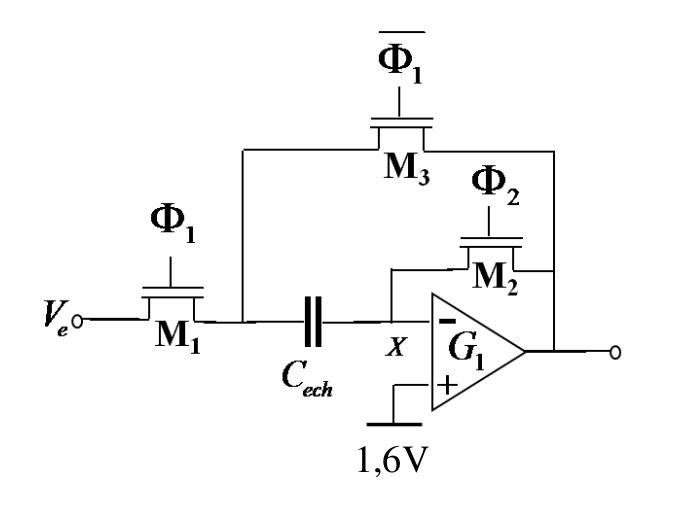
\includegraphics[scale=0.30]{Echantillonneur-bloqueur.jpg}
  \caption{Sch\'ema d'un \'echantilloneur-bloqueur \`a capacit\'e commut\'ee}
\end{center}
\end{figure}

\subsection{Principe de fonctionnement}

On rappelle qu'on a introduit un d\'ecalage entre les 2 horloges ($\Phi_1$ et $\Phi_2$) de 5 ns, sachant que la
fr\'equence d'\'echantillonnage est de $20 MHz$.

\begin{wrapfigure}{r}{0.5\textwidth}
\begin{center}
  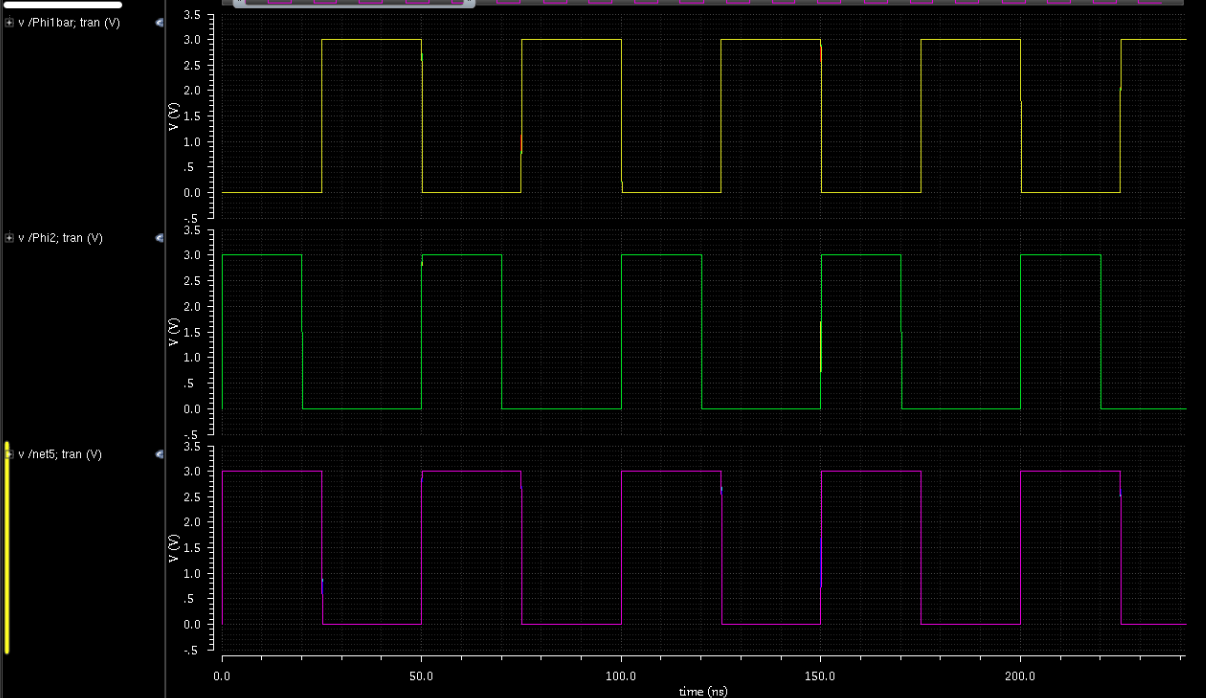
\includegraphics[width=0.55\textwidth]{clocks_.png}
\end{center}
\caption{Horloges de candencement}
\end{wrapfigure}

\medskip
L'echantillonneur bloqueur fonctionne en 2 r\'egime diff\'erents:
\begin{itemize}
  \item[-]\textbf{Phase m\'emoire} : C'est l'\'etape o\`u l'echantillonneur bloqueur
  reste sur la m\^eme valeur de tension en sortie pendant une dur\'ee T.
  \item[-]\textbf{Phase suiveur} : L'\'echantillonneur suit la variation d'entr\'ee.
\end{itemize}

Gr\^ace \`a la phase m\'emoire, l'\'echantillonneur permet de garder un niveau de tension
fixe pour la conversion qui suit.

Les sch\'ema \'electriques correspondant aux phases sont repr\'esent\'es par la figure \ref{fig:figEBfonct}.

\clearpage

\begin{figure}[!htb]
  \begin{subfigure}[t]{.5\linewidth}
      \centering
      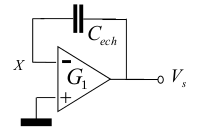
\includegraphics[width=0.6\linewidth]{memoire_EB.png}
      \caption{Phase de m\'emorisation}
      \label{fig:sfigEBmem}
  \end{subfigure}%
  \begin{subfigure}[t]{.5\linewidth}
    \centering
    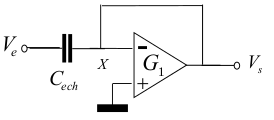
\includegraphics[width=0.6\linewidth]{suiveur_EB.png}
    \caption{Phase suiveur}
    \label{fig:sfigEBsuiv}
  \end{subfigure}%
  \caption{Diff\'erentes phases de fonctionnement de l'EB}
  \label{fig:figEBfonct}
\end{figure}

\begin{itemize}
  \item[-]\textbf{Phase m\'emoire} : On a $\overline{\Phi_1}$ et $\overline{\Phi_2}$, $\Phi_2 = 0$.\\
  $C_{ech}$ renvoie sa valeur de la charge en sortie.
  \item[-]\textbf{Phase suiveur} : On est \`a $\Phi_1$ et $\Phi_2$.\\
  Sachant que l'amplificateur OTA, plac\'e en suiveur, a une tr\`es grande imp\'edance d'entr\'ee, on a $V_{e^{+}} = V_{e^{-}}$.\\
  $C_{ech}$ prend la chage correspondante \`a $V_e - 1.5 V = V_e - \frac{V_{dd}}{2}$.
 \end{itemize}

Le d\'ecalage entre $\Phi_1$ et $\Phi_2$ entraine certainement le passage du transistor $M_1$ \`a l'\'etat ``Off'' avant le transitor
$M_2$. Par rapport \`a l'injection des charges, la haute imp\'edance d'entr\'ee de l'amplificateur \'elimine cet effet au niveau
de la capacit\'e $C_{ech}$, pendant le passage du MOS $M_1$ \`a l'\'etat ``Off''.

Pendant la phase interm\'ediaire o\`u on a $\Phi_1$ et $\overline{\Phi_2}$, le passage du MOS $M_2$ \`a l'\'etat ``Off'' entraine
l'injection des charges dans $C_{ech}$, mais celle-ci est constante du fait que $V_{e^{-}} = cte$.

Le gain du minimal \'etait sup\'erieur \`a 300, pour une adaptation avec la r\'esolution de 6bits. Ce gain sera v\'erifi\'e
dans la section \ref{OTA_sect}.

\subsection{Simulation avec des \'el\'ements id\'eaux}

\begin{figure}[!htb]
\begin{center}
  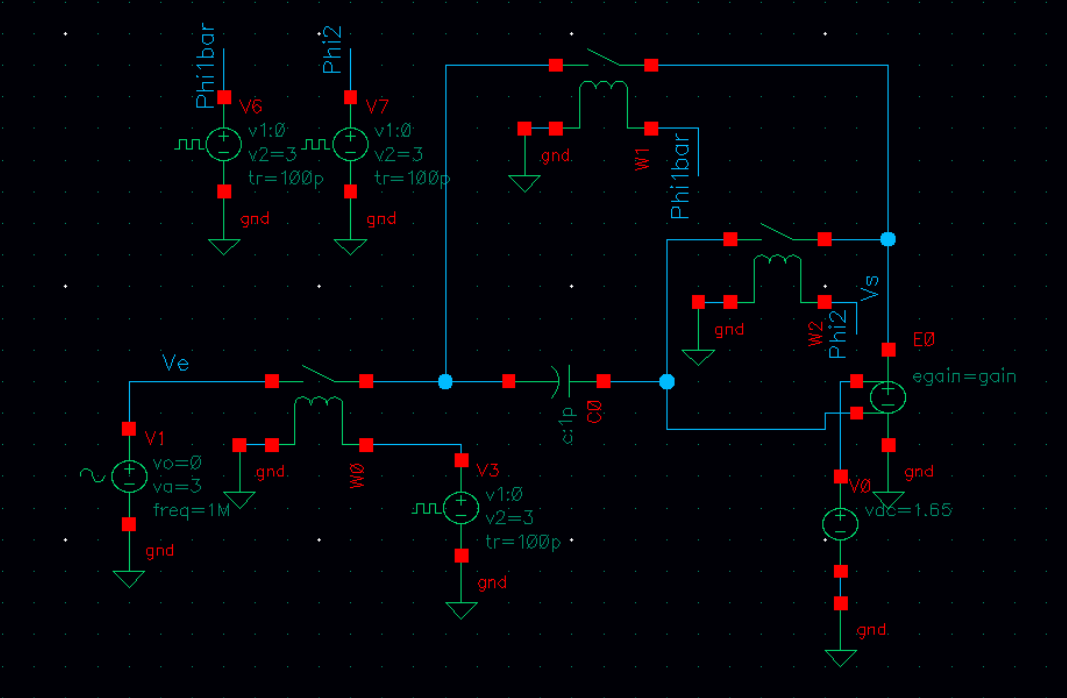
\includegraphics[scale=0.30]{Echantillonneur-bloqueur_ideal.png}
  \caption{Sch\'ema de l'\'echantilloneur-bloqueur en \'el\'ements ideaux}
\end{center}
\end{figure}

\clearpage

On configure les horloges avec le d\'ecalage pr\'evu, et on choisi d'effectuer
une analyse transitoire pour un signal d'entr\'ee sinuso\"idal de fr\'equence
$f = 1 MHz$ et de variation $V_e \in [-3, 3\phantom{1}V]$, la plage de variation
de 0.5 \`a 2.5 V n'est pas prise en consid\'eration pour le moment.

En g\'en\'eral, toute les simulations effectu\'ees pendant le project sont en analyse
transitoire, avec une dur\'ee de $1 \mu s$.

\begin{figure}[!htb]
\begin{center}
  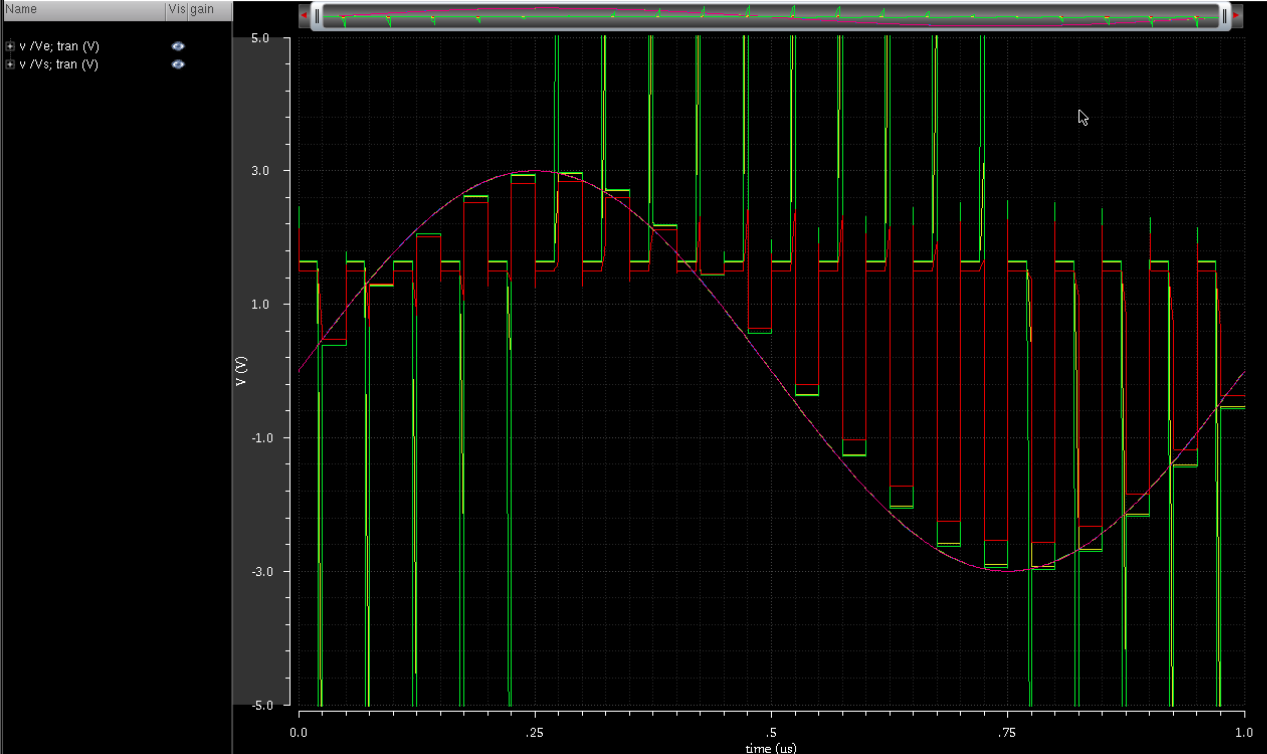
\includegraphics[width=0.8\linewidth]{simu_ech_bloqueur.png}
  \caption{Simulation transitoire l'\'echantilloneur-bloqueur id\'eal}
\end{center}
\end{figure}

Cette simulation prend en charge une variation d'un param\`etre ``gain'' de l'amplificateur
pour observer le chagement de niveau de tension en sortie du signal \'echantillonn\'e
en comparaison avec celui d'entr\'ee. On trouve qu'on a une meilleur approximation pour une
valeur de gain de l'amplificateur assez \'el\'ev\'ee.

\begin{figure}[!htb]
\begin{center}
  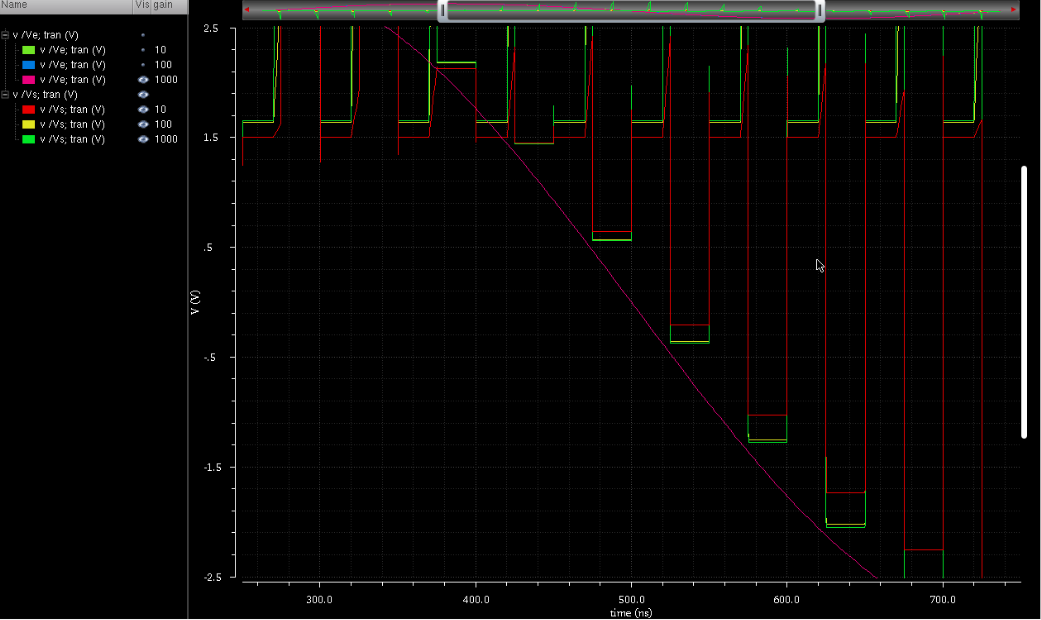
\includegraphics[width=0.76\linewidth]{rapport_gain_bloquage.png}
  \caption{Rapport gain-bloquage au niveau de l'\'echantilloneur-bloqueur id\'eal}
\end{center}
\end{figure}

\clearpage

\subsection{R\'ealistation des switchs r\'eels et simulations}

\textbf{Vue th\'eorique et Dimensionnements}

La mise en place d'un \'echantillonneur bloqueur n\'ecessite la r\'ealisation
des switch en CMOS.

Du point du vue th\'eorique, un switch est une mise en parall\`ele de 2 transistors
de type PMOS et NMOS (TGATE).

\begin{figure}[!htb]
  \begin{subfigure}[t]{.5\linewidth}
      \centering
      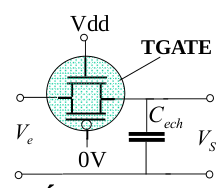
\includegraphics[width=0.7\linewidth]{tgate_.png}
      \caption{Structure du TGate}
      \label{fig:sfigtgate}
  \end{subfigure}%
  \begin{subfigure}[t]{.5\linewidth}
    \centering
    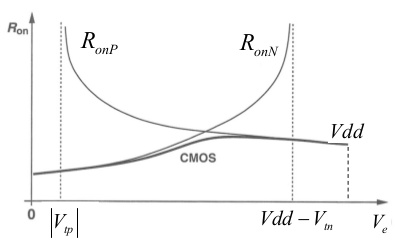
\includegraphics[width=0.9\linewidth]{var_ron.png}
    \caption{Variation des $R_{ON}$ des MOS en fonction de $V_e$}
    \label{fig:sfigron}
  \end{subfigure}%
  \caption{}
  \label{fig:figswitchth}
\end{figure}

Ces switchs seront dimmensionn\'es pour respect\'e le temps de charge de C
correspondante \`a la fr\'equence d'\'echantillonnage de $20 MHz$. On choisi alors
une constante de temps $\tau$ assez r\'eduite.

\begin{figure}[!htb]
\begin{center}
  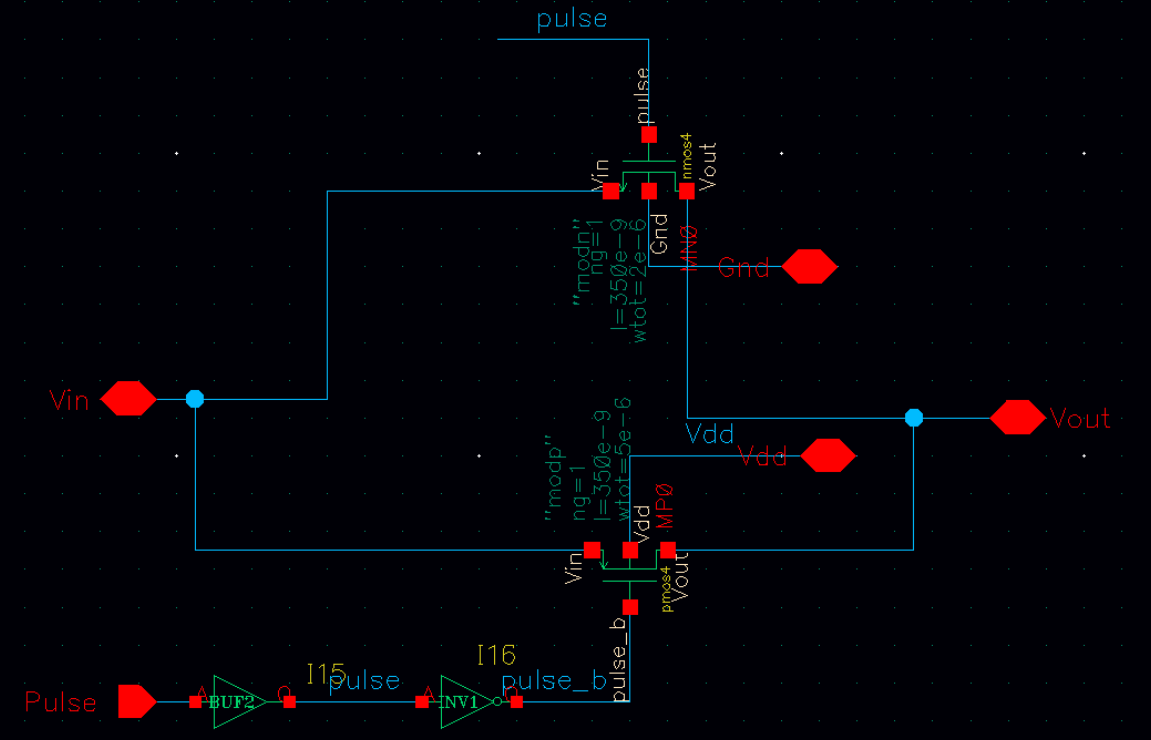
\includegraphics[width=0.8\linewidth]{switchs_.png}
  \caption{Sch\'ema \'electrique des switchs en CMOS}
\end{center}
\end{figure}



\clearpage

Si les transistors MOS se comportent comme des r\'esistances en parall\`ele,
il est possible de calculer $R_{ON} = R_{ON_{(P)}}//R_{ON_{(N)}}$.
Les transistors on \'etait dimmensionn\'es pour une $C_{ech} = 7 pF$
\[
  \tau = R_{ON} C \implies R_{ON} = \frac{\tau}{C} = \frac{1}{200\times10^{6}\times7\times10^{-12}} = 714.28 \Omega
\]
Sachant que $\tau << \frac{1}{F_e} = \frac{1}{20\times10^6} s$, on prend $\tau = \frac{1}{200 \times 10^6} s$.

\[
  R_{ON} = R_{ON_{(P)}}//R_{ON_{(N)}} \implies \frac{1}{R_{ON}} = \frac{1}{ R_{ON_{(P)}}} + \frac{1}{ R_{ON_{(N)}}}
\]

On prend $  R_{ON_{(P)}} =  R_{ON_{(N)}} \implies  R_{ON_{(P)}} = 2 R_{ON} = 1428 \Omega$

Pour les 2 transistors :
\[
R_{ON_{(N)}} = \frac{1}{2k_n \frac{W}{L} (V_{GS} - V_{tn})} \phantom{2} et \phantom{2} R_{ON_{(P)}} = \frac{1}{2k_p \frac{W}{L} (V_{SG} - V_{tp})}
\]

D'o\`u : (Pour $V_{e}$ d'entr\'ee $ = \frac{V_{dd}}{2}$, on se place au milieu de la dynamique (fig.\ref{fig:sfigron}))
\[
\bigg(\frac{W}{L}\bigg)_{N} = \frac{1}{2k_n R_{ON_{(N)}}  (V_{GS} - V_{tn})} =\frac{1}{2k_n R_{ON_{(N)}}  (\frac{V_{DD}}{2} - V_{tn})} = 5.71 \implies (W)_{N} = 2 \mu m.
\]

\[
\bigg(\frac{W}{L}\bigg)_{P} = \frac{1}{2k_p R_{ON_{(P)}}  (V_{SG} - V_{tp})} = \frac{1}{2k_p R_{ON_{(P)}}  (\frac{V_{DD}}{2} - V_{tp})} = 14.48 \implies (W)_{P} = 5 \mu m,  L_{P} = 0.35 \mu m.
\]

\textbf{V\'erification des performances par simulations}

\begin{figure}[!htb]
\begin{center}
  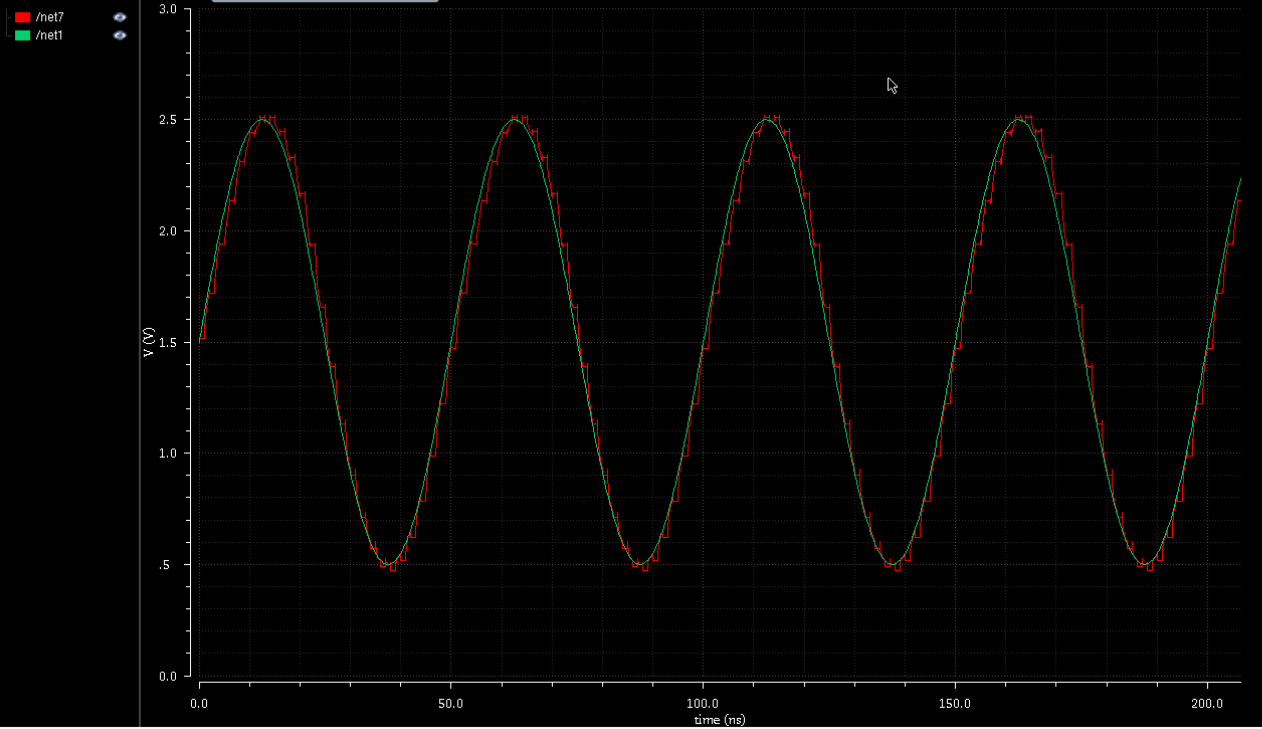
\includegraphics[width=0.8\linewidth]{switchs_simu.png}
  \caption{Simulation des switchs}
\end{center}
\end{figure}

La commutation des switchs est assez rapide par rapport \`a la fr\'equence du signal d'entr\'ee.

\clearpage

\subsection{Simulation finale}
En rassemblant tous les \'el\'ements, on aboutit au sch\'ema suivant :

\begin{figure}[!htb]
\begin{center}
  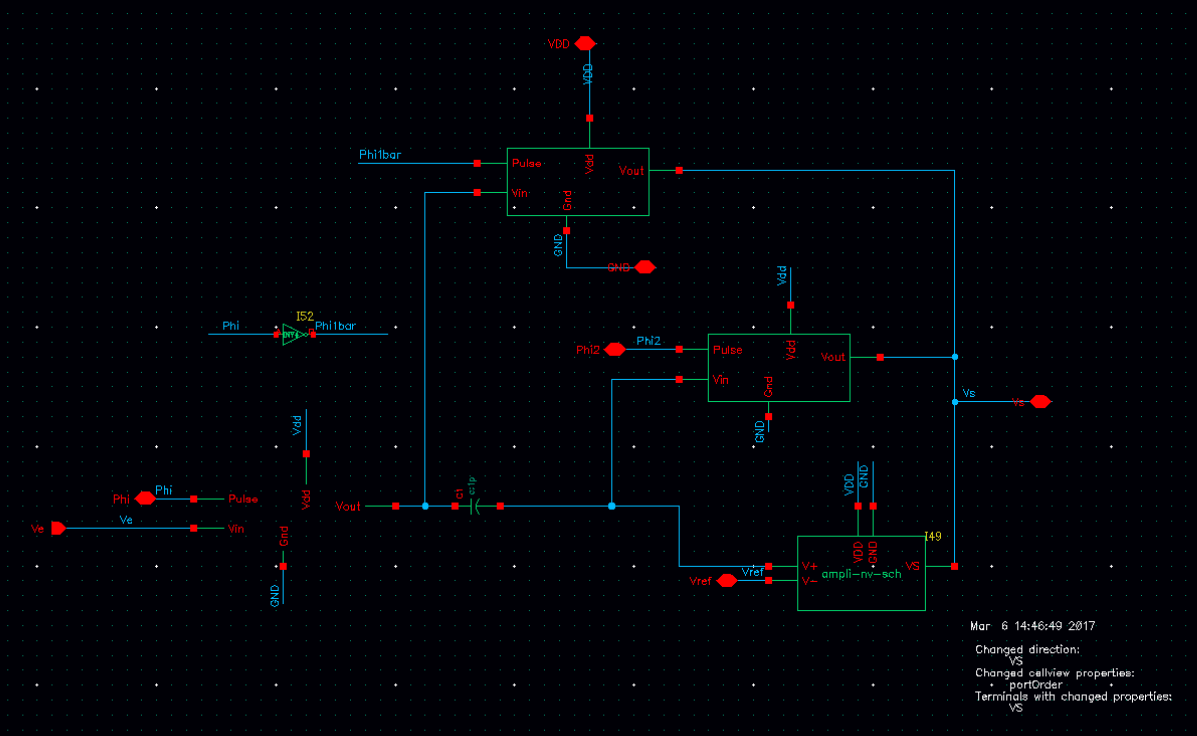
\includegraphics[width=0.80\linewidth]{EB-Schematic.png}
  \caption{Sch\'ema de l'\'echantilloneur-bloqueur r\'eel}
\end{center}
\end{figure}

Effectuant la simulation :

\begin{figure}[!htb]
\begin{center}
  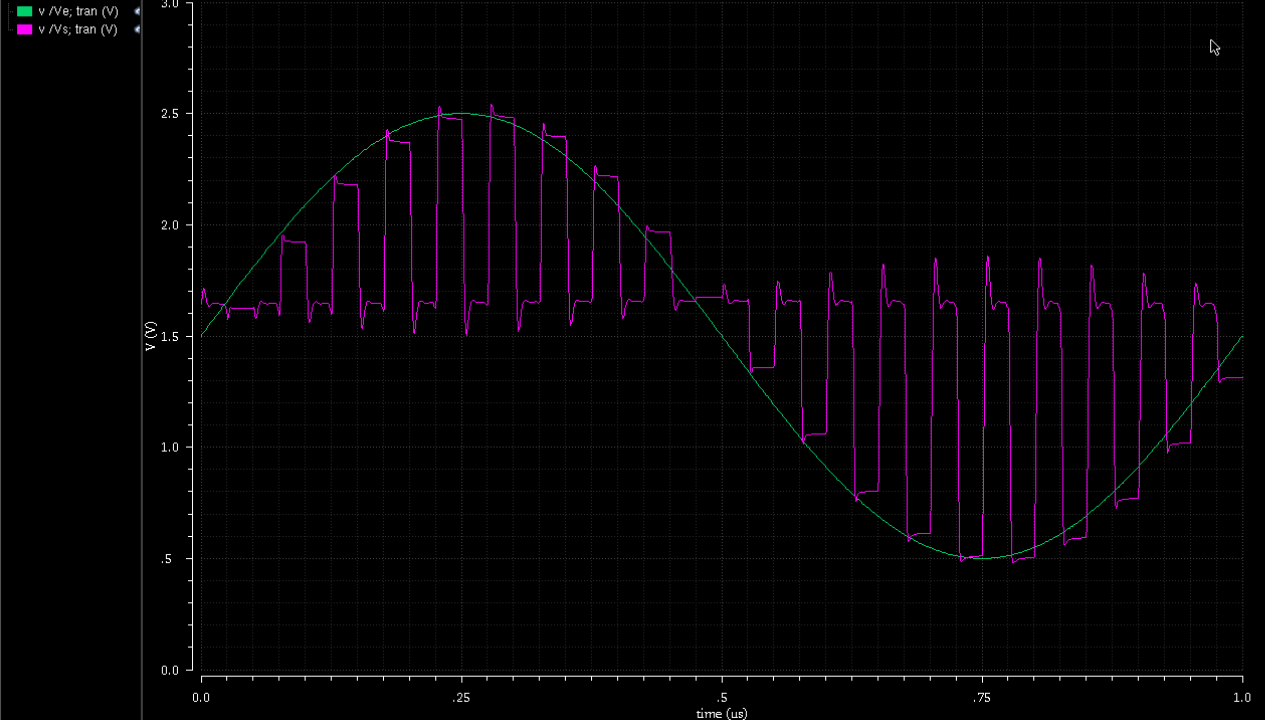
\includegraphics[width=0.80\linewidth]{simu_ech_bloqueur_reel.png}
  \caption{Simulation de l'\'echantilloneur-bloqueur r\'eel}
\end{center}
\end{figure}

On rappelle que la mise en place de tous le \'el\'ements n\'ecessite la pr\'esence d'un amplificateur
r\'eel, fonctionnant comme suiveur. Cet \'el\'ement est expliqu\'e dans la section suivante (sect. \ref{OTA_sect}). On voit alors un comportement tr\`es similaire au celui de l'\'echantillonneur-bloqueur pr\'e-dimensionn\'e, avec un gain pr\'evu, pour une dynamique d\'entr\'ee de $V_e \in [0.5; 2.5 V] $.

\clearpage
\section{R\'ealisation d'un Amplificateur OTA \`a deux \'etages}\label{OTA_sect}

\subsection{Cahier des charges}

\textbf{Le cahier de charges n\'ecessite :}
\begin{itemize} \itemsep -4pt
  \item[-] Un gain minimal pour une r\'esolution de 6 bits : $G(0) = 300$
  \item[-] Dynamique en entr\'ee de $V_e \in [0.5, 2.5 V]$
  \item[-] Puissance : $P = 2mW$
  \item[-] Dynamique en sortie : $V_S \in [0.5, 3.5 V]$
    \item[-] Fr\'equence maximale d'op\'eration $~ 180 MHz$
\end{itemize}

\subsection{Calcul th\'eorique et dimensionnements}

Le calcul th\'eorique et la prise en compte du dimensionnement nous am\`ene au sch\'ema
suivant :

\begin{figure}[!htb]
\begin{center}
  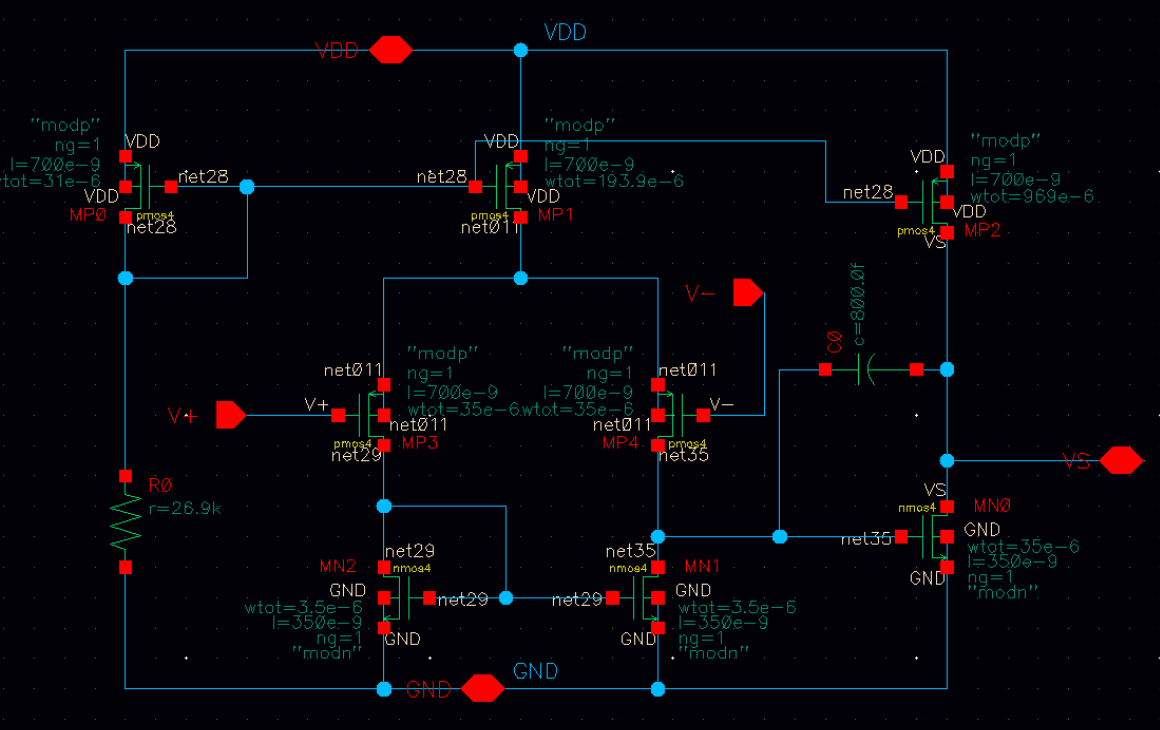
\includegraphics[width=\linewidth]{amplificateur_.png}
  \caption{Architecture de l'amplificateur \`a deux \'etages apr\`es dimensionnements}
\end{center}
\end{figure}

Les calculs, ainsi que le principe de fonctionnement, sont d\'etaill\'es dans l'annexe 1 (sect. \ref{Annexe1}). 
 
\clearpage

\subsection{Simulation et optimisation}

\begin{figure}[!htb]
\begin{center}
  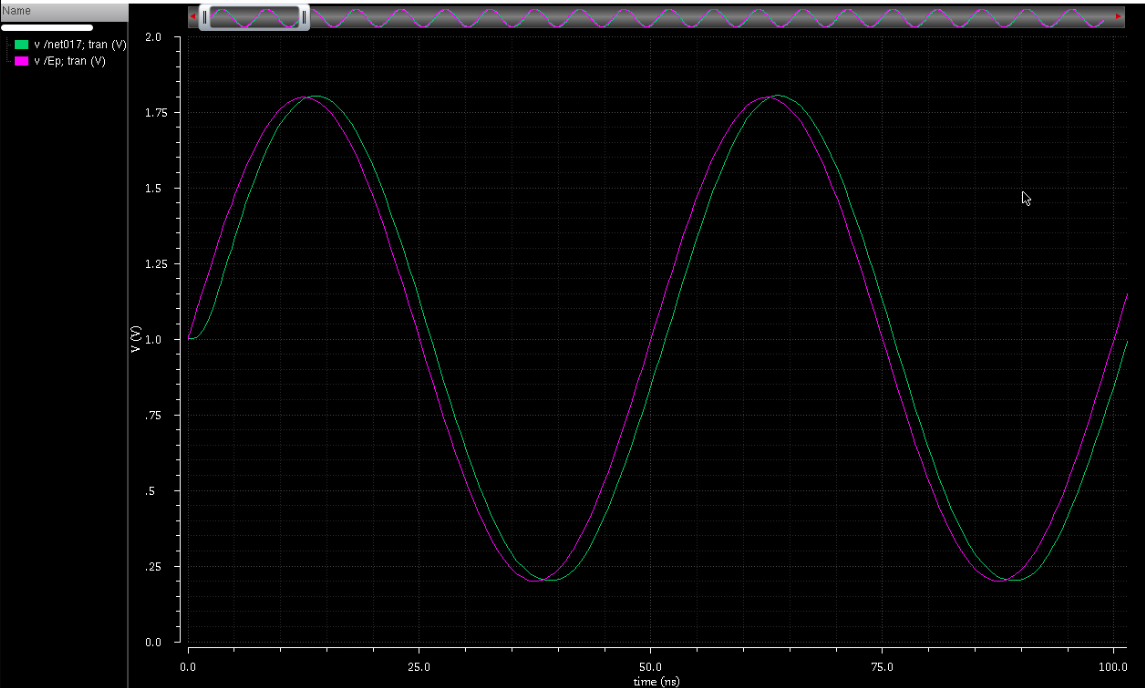
\includegraphics[width=0.85\linewidth]{reponse_ampli.png}
  \caption{Simulation de l'amplificateur en r\'egime transitoire}
  \label{fig:figSimAmp}
\end{center}
\end{figure}

La figure \ref{fig:figSimAmp} montre la simulation de l'amplificateur tout seul, avec une entr\'ee
sinuso\"idale. On trouve alors un d\'ephasage entre l'entr\'ee et la sortie par rapports aux
caract\'eristiques choisies.

\begin{figure}[!htb]
\begin{center}
  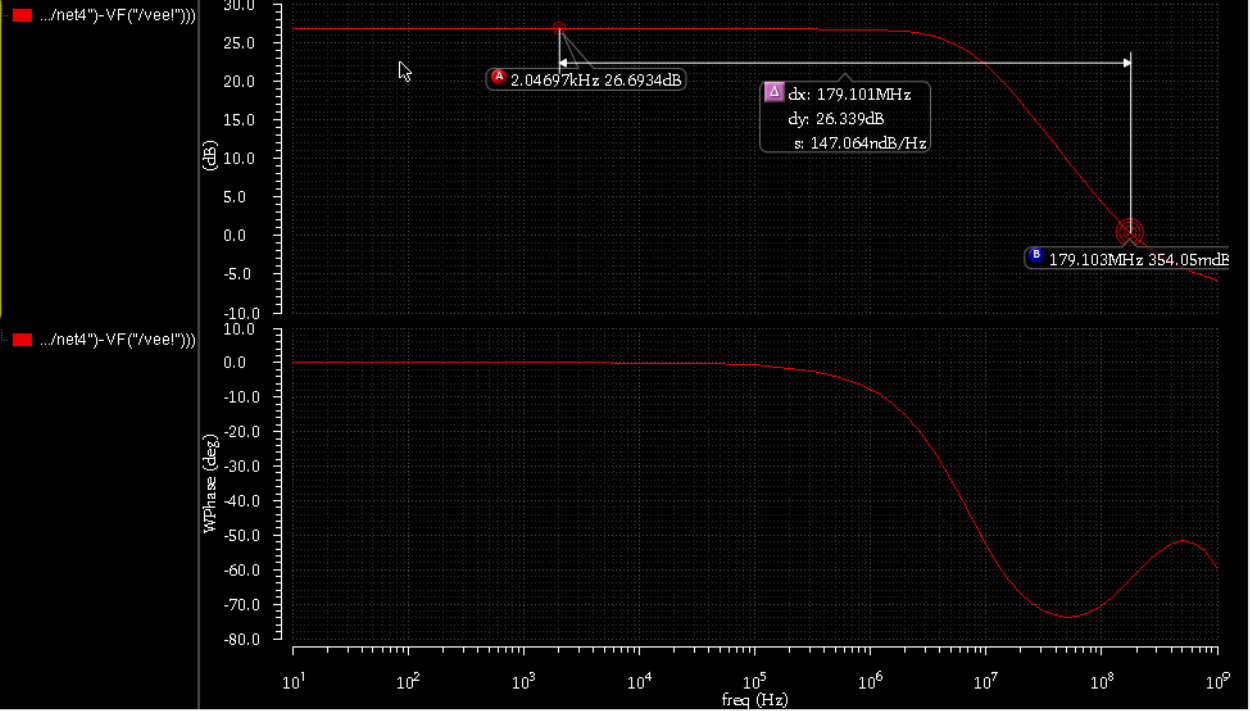
\includegraphics[width=0.85\linewidth]{sim_EB_freq.png}
  \caption{Simulation en \'etude AC  de l'amplificateur (comportement fr\'equentiel)}
  \label{fig:figSimAmpAC}
\end{center}
\end{figure}

La simulation AC montre que l'amplificateur pr\'esente un comportement assimilable \`a un filtre passe-bas, \`a une fr\'equence de coupure autour de 10 MHz, avec une marge de phase de -60 degr\'ees autour de cettre fr\'equence. L'att\'enuation maximale de (-26 dB) est atteinte \`a 180 MHz.

\clearpage

\section{Mise en oeuvre des comparateurs synchronis\'es par horloge}
\subsection{Principe de fonctionnement}
L'\'etape suivante est la cr\'eation de 63 comparateurs et seuils afin d'au mieux \'evaluer le niveau de
notre signal \`a chaque front sur un cycle d'horloge commune \`a tous les blocs.

\begin{figure}[!htb]
\begin{center}
  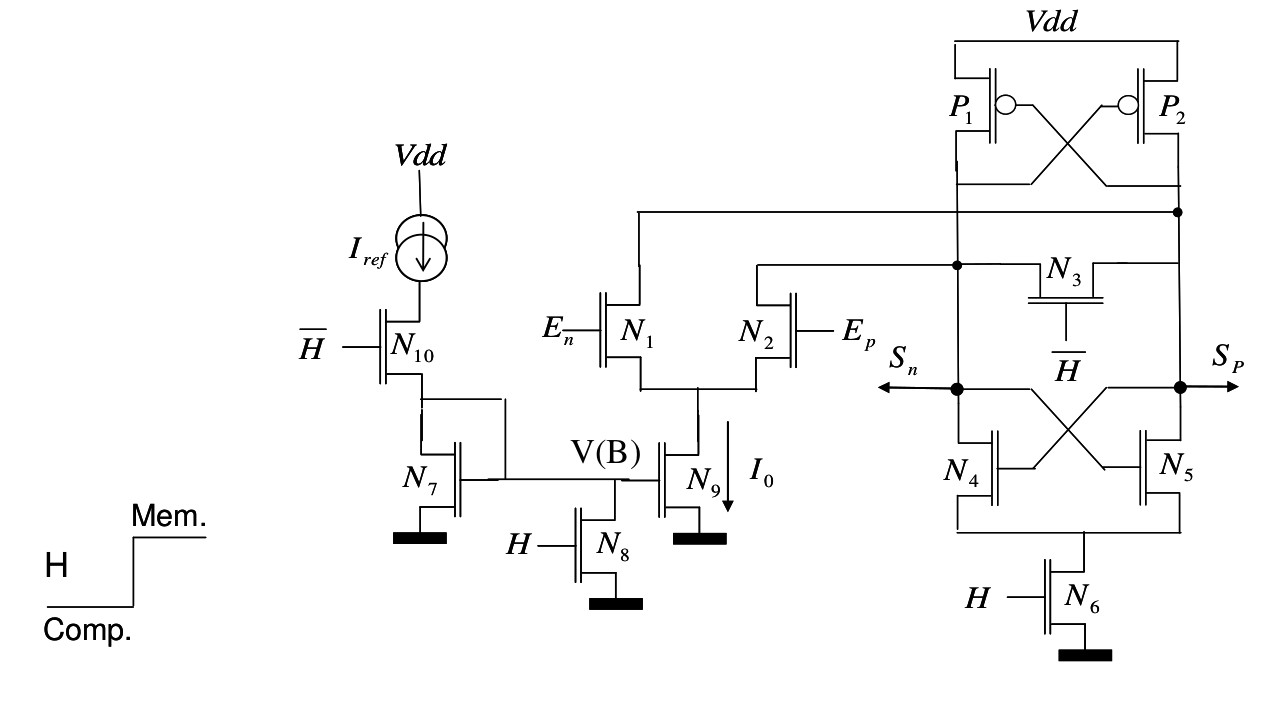
\includegraphics[scale=0.38]{comparateur_schema.jpg}
  \caption{Architecture des comparateurs synchronis\'es par horloge avec une paire crois\'ee}
  \label{fig:figArchComp}
\end{center}
\end{figure}

La structure utilis\'ee pour ce comparateur et bri\`evement d\'ecrite dans le sujet, et illustr\'ee par
la figure \ref{fig:figArchComp}, utilise un courant provenant d'un miroir de courant (partie gauche de la structure).
La propri\'et\'e comparatrice est effectu\'ee par la paire diff\'erentielle $N_1$/$N_2$ Ensuite, la partie de droite
($P_1$,$P_2$ et $N_3$,$N_4$,$N_5$,$N_6$) fait basculer le comparateur soit en satur\'e (sortie de 3.3 V)
ou \`a la masse \`a travers le transistor $N_6$ qui est alors passant.

\subsection{Partie Th\'eorique}
Afin d'au mieux dimensionner ce comparateur, nous avons effectu\'e les hypoth\`eses et calculs suivants,
par rapport au courant et aux dimensions des transistors:

\subsubsection{Phase de comparaison (niveau d'horloge bas)}

Pour $V_{EP}-V_{EN}$ tr\`es diff\'erent de $0$ (cas d'une entr\'ee repr\'esentant le signal et l'autre un seuil),
le courant $I_0$ capable de charger ou d\'echarger la capacit\'e aux nœuds $S_N$ ou $S_P$ en $\frac{1}{4}$ de
p\'eriode d'horloge sur une variation de $V_{DD}$ vaut :

\[
I_0 = C \frac{V_{DD}}{t} = 26 \mu A
\]

si l'on consid\`ere un temps de 12.5 ns = $\frac{1}{4} \times T_{horloge}$ \`a 20 MHz.

A l'\'equilibre ($V_{EN} = V_{EP}$), pour avoir une tension de mode commun en sortie
$V_{SN} = V_{SP} = \frac{V_{DD}}{2}$ , le rapport $\frac{W}{L}$ de $P_{1,2}$ vaut :

\[
  \bigg(\frac{W}{L}\bigg)_{P1,2} = \frac{I_D}{K_P (V_{dd}/2 - |V_{TP}|)^{2}} = 1.229
\]

Afin que les transistors $N_{1,2}$ pr\'esentent une capacit\'e $C_{GS}$ en entr\'ee compatible
ou inf\'erieure \`a celle prise en compte pour fixer $C_s$ dans le calcul de l'\'echantillonneur
bloqueur, la relation :

\[
  C_{GS} = \frac{2}{3} C_{ox} W_{N_{1,2}} L \leq C_{comp}
\]

Ce qui implique que $W_{N_{1,2}} \leq 68 \mu m$ puisque :

\[
  C_S = C_{ech} + 63 \times C_{comp}
\]
et que :
\[
  C_{comp} = \frac{5}{63} \phantom{2} pF = 79 fF
\]

D\'eterminons maintenant les tailles des transistors servant \`a polariser la paire N1/N2 :

Si l'on remplace $N_{9}$ par un g\'en\'erateur de courant de valeur $I_{0}$, une simulation DC
sous Cadence donne une valeur de tension au noeud A : $V_A = 0.75 V$.

Afin que la grille du transistor $N_9$ soit polaris\'e avec la condition $V_{GS}-V_{tn}=V_{DS} - 0,2V$
 (0,2V au-dessus de la limite de zone active), nous en d\'eduisons la tension au noeud B : $V_B = 1.12 V$

Puis, le calcul de $\frac{W}{L}$ de $N_9$ vient avec :
\[
  I_d = K_n \frac{W}{L} (V_{gs} - V_{tn})^2 \bigg( 1 + \frac{K_{en}}{L} V_{ds}\bigg)
\]

Le transistor est au-dessus de la LZA :

\[
\bigg(\frac{W}{L} \bigg)_{N_9} = \frac {26µA}{55µA . (V_B - V_T)^2 ( 1+ (0.03/0.35) V_A)}
\]
\[
\bigg(\frac{W}{L} \bigg)_{N_9} = 1.46
\]

Nous faisons de m\^eme afin de calculer les dimensions du transistor $N_7$ avec la condition
$I_{ref} =\frac{I_0}{2}$

Pour calculer celui de N7, m\^eme formule sauf que :
\[
  \bigg(\frac{W}{L} \bigg)_{N_7} = \frac {\frac{26}{2}µA  }{55µA . (V_B - V_T)^2 ( 1+ (0.03/0.35) V_B)}
\]
\[
\bigg(\frac{W}{L} \bigg)_{N_7} = 0.72
\]

On prendra pour $N_{10}$ un $W = 5 \mu m$.

Le calcul des dimensions du transistor $N_8$ s'effectue en consid\'erant qu'il peut charger ou d\'echarger
la capacit\'e estim\'ee par simulation au noeud B en $\frac{1}{4}$ de p\'eriode d'horloge.

\[
I_{N_8} = \frac {V_B C_B}{\frac{1}{4} T_H} = 2 µA
\]

\iffalse
\textbf{\textcolor{red}{Mettre les simulations}}
\fi

\textit{Note} : On rappelle que pendant cette phase, le couple des PMOS $P_{1,2}$ du comparateur fonctionne comme une imp\'edance diff\'erentielle n\'egative\cite{Razavi-Data-Conversion}. On retrouve que si on consi\`ere cette branche seule, on a :
\[
\frac{V}{I}= -2 \frac{1}{g_m_{(P_{1,2})}} = -2 R_{ON}
\]


\subsubsection{Phase de m\'emorisation (niveau d'horloge haut)}

Afin que la chute de tension dans le transistor $N_6$  \`a l'\'etat ON soit de l'ordre de $0,5 V$ lorsque $H=1$
pour un courant $I_{N_6}= I_0$, il vient :
\[
  \bigg(\frac{W}{L} \bigg)_{N_6} = 0.19
\]

car la chute de tension \`a travers la r\'esistance ON du transistor vaut $R_{ON} \times I_0 = 0.5V$

Pour une tension de mode commun en sortie $V_{SP}=V_{SN} = \frac{V_{dd}}{2}$,

\[
  \frac{I_0}{2} = K_n \frac{W}{L}(1.65-0.5 - V_{tn})^2
\]
\[
  \bigg(\frac{W}{L} \bigg)_{N_{4,5}} = 0.70
\]

Le dimensionnement des transistors nous am\`ene au sch\'ema de la fig. \ref{fig:schcomp}.


\clearpage

\begin{figure}[!htb]
      \centering
      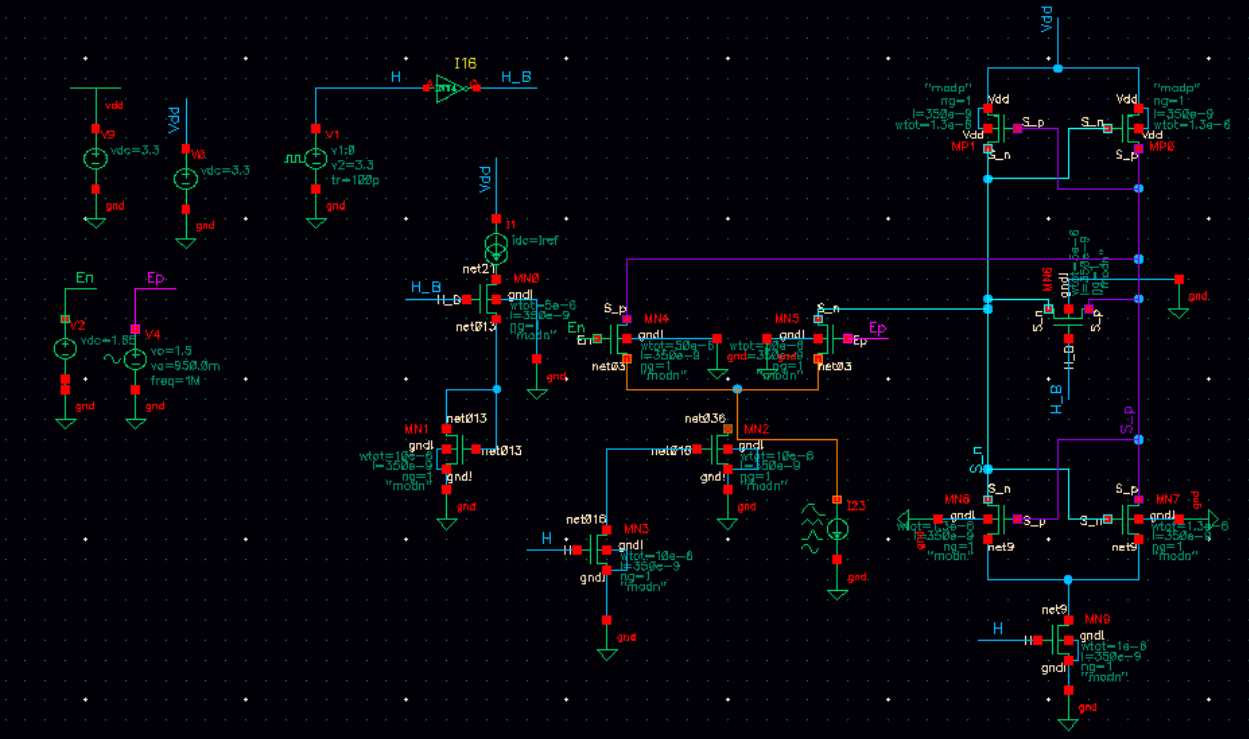
\includegraphics[width=0.8\linewidth]{comparateur_schema_cadence_.png}
      \caption{Sch\'ema \'electrique}
      \label{fig:schcomp}
\end{figure}%


\subsection{Simulations/Optimisations}

Finalement, les simulations pr\'esentent un comparateur qui est approximatif : la sortie en mode
commun n'est jamais r\'eellement soit \`a 0 ou \`a 3.3 V. En effet, le z\'ero logique se situe autour de 0 et 1 V
et le 1 logique varie entre 2.5 et 3.3 V. \iffalse \textbf{\textcolor{red}{Sch\'ema ne correpsond pas \`a la description, simulation
\`a refaire avec le bon dimensionnement du comporateur (dernier comp)}} \fi

\begin{figure}[!htb]
      \centering
      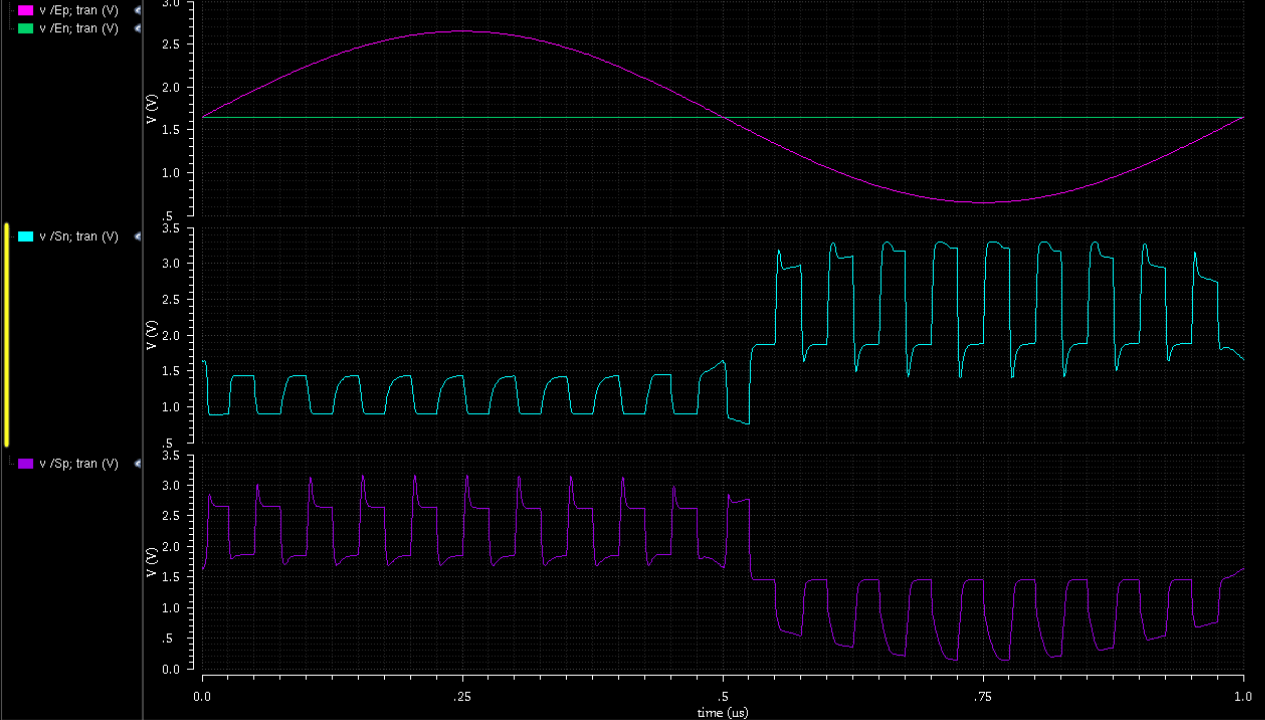
\includegraphics[width=0.8\linewidth]{simu_comp_pas_ameliore.png}
      \caption{Simulation avant l'ajout des buffers + bascules}
      \label{fig:sfigBSRFF}
\end{figure}%

Nous avons donc rajout\'e des inverseurs et une Bascule SR (en 2 Nandes interconnect\'ees) en sortie afin de m\'emoriser un 0 ou un 1 logique. Ces \'el\'ements sert \`a garder un niveau stable pendant la commutation de l'horloge.

\begin{figure}[!htb]
      \centering
      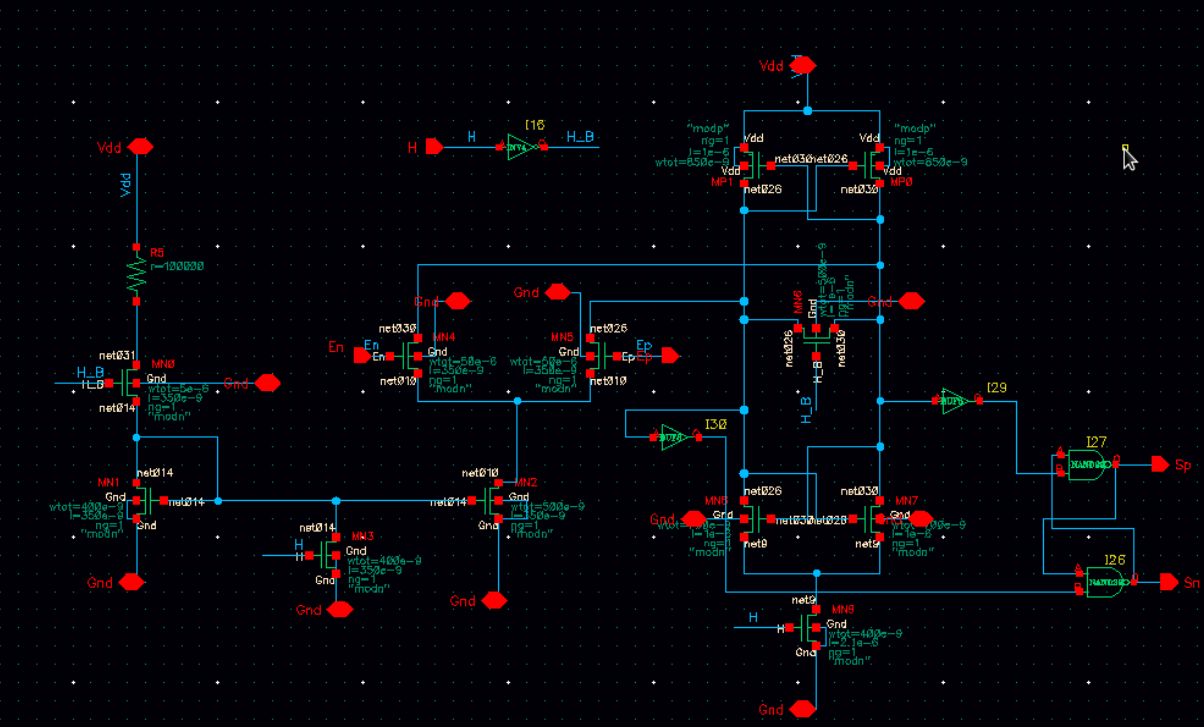
\includegraphics[width=0.9\linewidth]{comparateur_schema_cadence_SR.png}
      \caption{Sch\'ema \'electrique}
      \label{fig:schcompSR}
\end{figure}%

\begin{figure}[!htb]
      \centering
      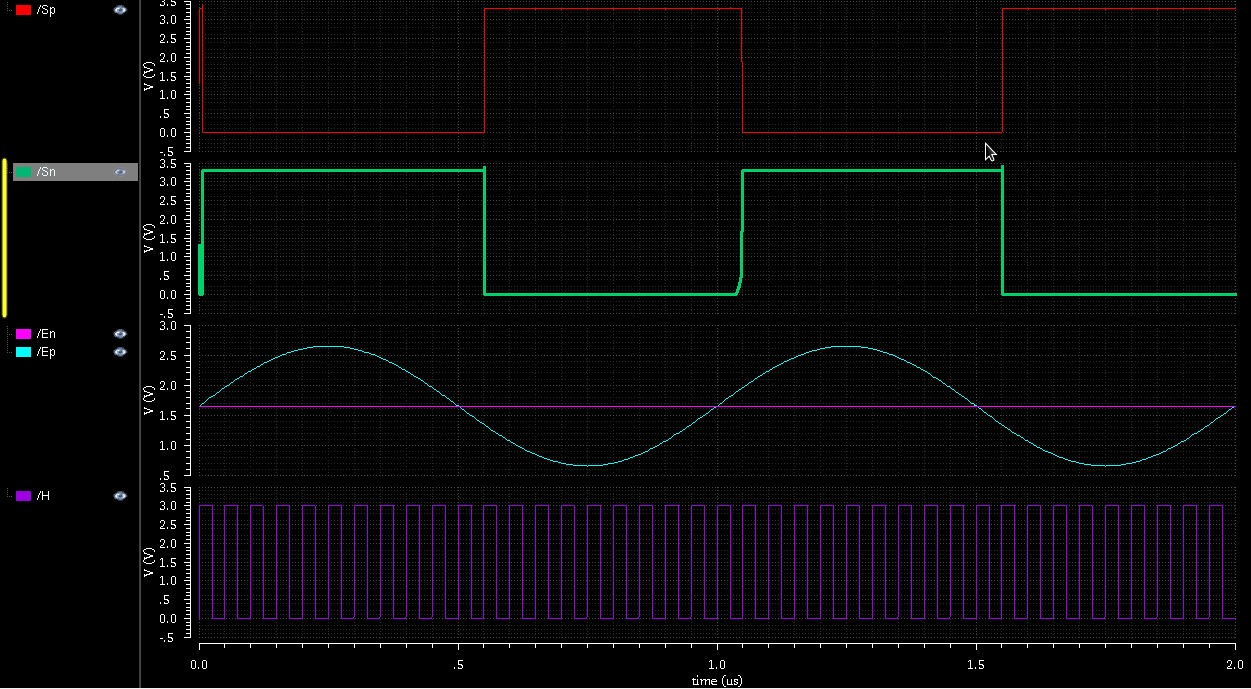
\includegraphics[width=\linewidth]{sim_comp_after_SR_FF.jpg}
      \caption{Simulation apr\`es l'ins\'ertion de ces \'el\'ements}
      \label{fig:sfigASRFF}
\end{figure}%


\iffalse
\begin{figure}[!htb]
  \begin{subfigure}{.5\textwidth}
      \centering
      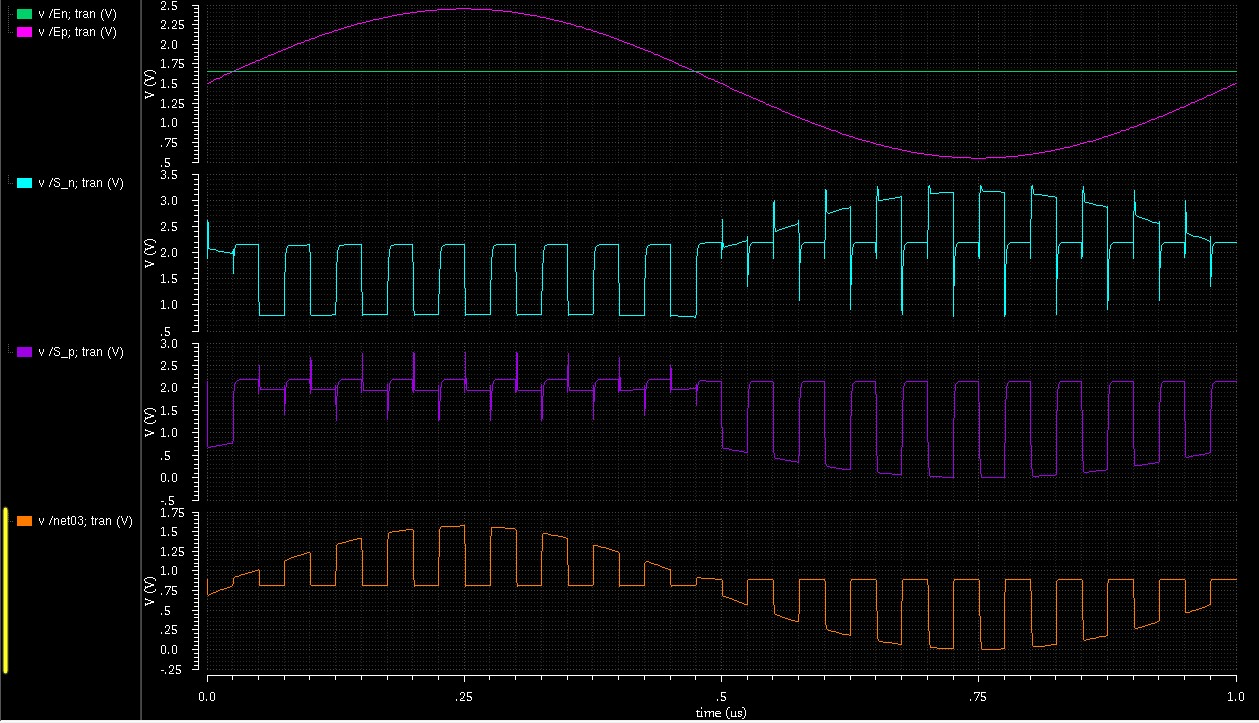
\includegraphics[width=1.2\linewidth]{sim_comp_before_SR_FF.jpg}
      \caption{Simulation avant l'ajout des buffers + bascules}
      \label{fig:sfigBSRFF}
  \end{subfigure}%

  \begin{subfigure}{.5\textwidth}
    \centering
    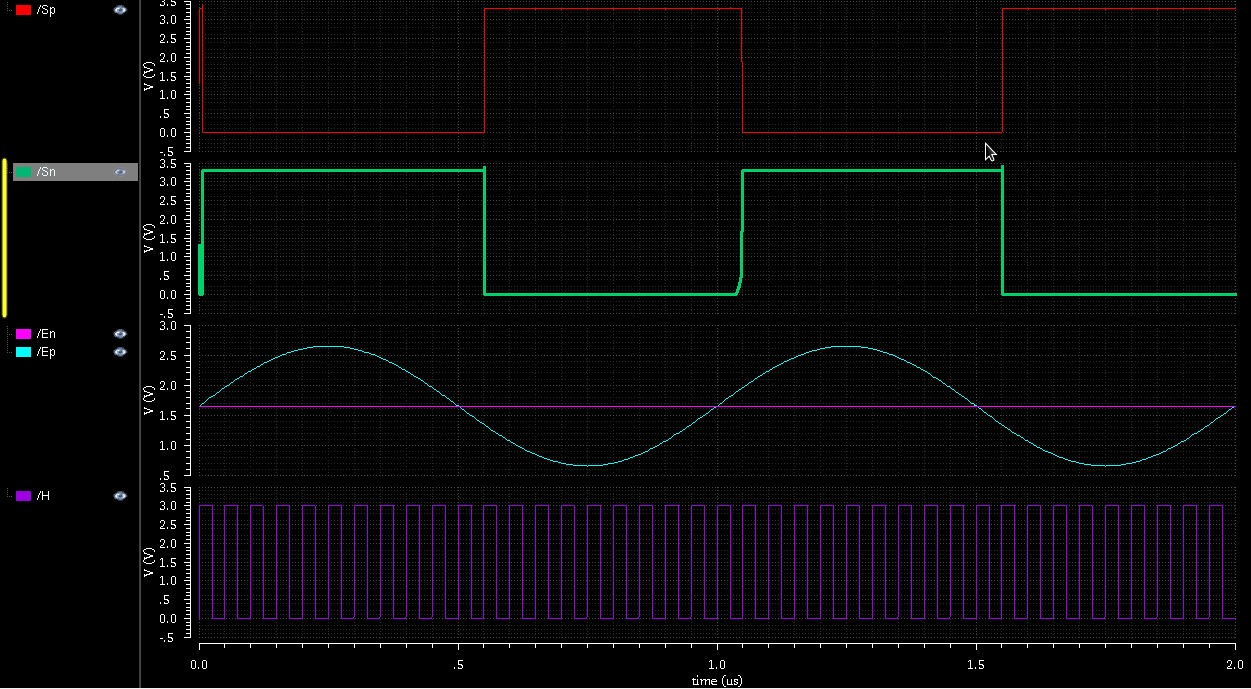
\includegraphics[width=1.2\linewidth]{sim_comp_after_SR_FF.jpg}
    \caption{Simulation apr\`es l'ins\'ertion de ces \'el\'ements}
    \label{fig:sfigASRFF}
  \end{subfigure}

  \caption{Diff\'erence en sortie en simulation entre comparateurs sans/avec bascule SR respectivement}
  \label{fig:figcomp}
\end{figure}
\fi

\iffalse
\subsubsection{Imp\'edance diff\'erentielle n\'egative et expression du Gain}
\subsubsection{D\'etermination du courant et dimensionnements}
\fi

\clearpage

\section{R\'ealisation du d\'ecodeur en Verilog}
\subsection{Programmation et synth\`ese automatique du circuit}
On utilise un code existant en Verilog\cite{Thermometer}.
Ce code permet de convertir les donn\'ees en code thermometrique en sortie des
comparateurs vers un code binaire sur 6 bits (avec un pouvoir de pr\'evention de bulles).

\begin{lstlisting}[language=Verilog, belowskip=-0.5 \baselineskip]
module thermo2bin (thermob, bin)
input[62:0] thermob;
output [5:0] bin;

reg [62:0] thermo;
reg [5:0] bin, bin1, bin2;
integer i, j, k;

always @(thermob)
begin
  for (k = 0; k <=60; k=k+1)
    thermo[k] <= thermob[k] || thermob[k+1] || thermob[k+2];

  thermo[61] <= thermob[61] || thermob[62];
  thermo[62] <= thermob[62];
end

always @(thermo)
begin
  bin1 = 0;
  for(i=1; i <= 32; i=i+1)
    if (thermo[i-1] = 1'b1) bin1 = i;
end

always @(thermo)
begin
  bin2 = 0;
  for(j=1; j<=31; j=j+1)
    if(thermo[k+31] == 1'b1) bin2 = j;
end

always @(bin1 or bin2)
if (thermo[31] == 1'b1)
  bin = bin2 + 32;
else
  bin = bin1;

endmodule

\end{lstlisting}

\subsubsection{Fonctionnement}

Ce module fonctionne du m\^eme principe de la lecture humaine : On essaye de lire le plus
haut '1'. Ce bout de code \'etait optimis\'e pour qu'il fonctionne en 2 parties pour optimiser
le chemin critique r\'esultant du circuit en synth\`ese. 

La lecture se fait dans les boucles ``for'', o\`u on cherche le plus grand '1'.
\begin{lstlisting}[language=Verilog, belowskip=-2 \baselineskip]
 for(i=1; i <= 32; i=i+1)
    if (thermo[i-1] = 1'b1) bin1 = i;
\end{lstlisting}
Pour le premier segment, et
\begin{lstlisting}[language=Verilog, belowskip=-2 \baselineskip]
  for(j=1; j<=31; j=j+1)
    if(thermo[k+31] == 1'b1) bin2 = j;
\end{lstlisting}
pour le deuxi\`eme.

La d\'ecision se prend finalement sur :
\begin{lstlisting}[language=Verilog, belowskip=-2 \baselineskip]
if (thermo[31] == 1'b1)
  bin = bin2 + 32;
else
bin = bin1;
\end{lstlisting}
O\`u on ajoute 32 \`a la valeur finale si on d\'etecte le 1 dans le segment LSB (le deuxi\`eme),
et on prend la valeur du bin1 directement sinon (segment MSB).

\subsubsection{Synth\`ese}

Ce code \'etait v\'erifi\'e et simul\'e sous ModelSim, avec le test bench en Verilog visulis\'e ci-dessous. Pour faciliter son int\'egration sous Cadence, on lance l'outil design precision, et on le configure pour la technologie CMOS $0.35 \mu m$.

\begin{lstlisting}[language=Verilog, belowskip=-2 \baselineskip]
module thermo2bin_tb;
  reg [62:0] thermob;
  wire [5:0] bin;
	
  thermo2bin DUT (
    .thermob(thermob),
    .bin(bin)
   );
  initial begin
    #100
    thermob = 63'b000000000000000000000011111111111111111111111111111111111111111;
    #100
    thermob = 63'b000000000000000111111111111100111111111111111111111111111111111;
    #100
    thermob = 63'b000000000000000000000000000000000000000000000000000000000000000;
    #100
    thermob = 63'b000000000000000000000000000000000000000000000000000000000000001;
    #100
    thermob = 63'b000000000000000000000000000000000000000000000000000000000000100;	
    #100
    thermob = 63'b000000000000000000000000000000000000000000000000000000000000110;
    #100
    thermob = 63'b000000000000000000000000000000000000000000000000000000000000111;
    #100
    $finish;
  end
endmodule
\end{lstlisting}

\clearpage
\subsection{Simulations}

La v\'erification du comportement du code \'etait r\'ealis\'ee sous ModelSim, mais il fallait une
autre simulation sous Cadence :

\begin{figure}[!htb]
      \centering
      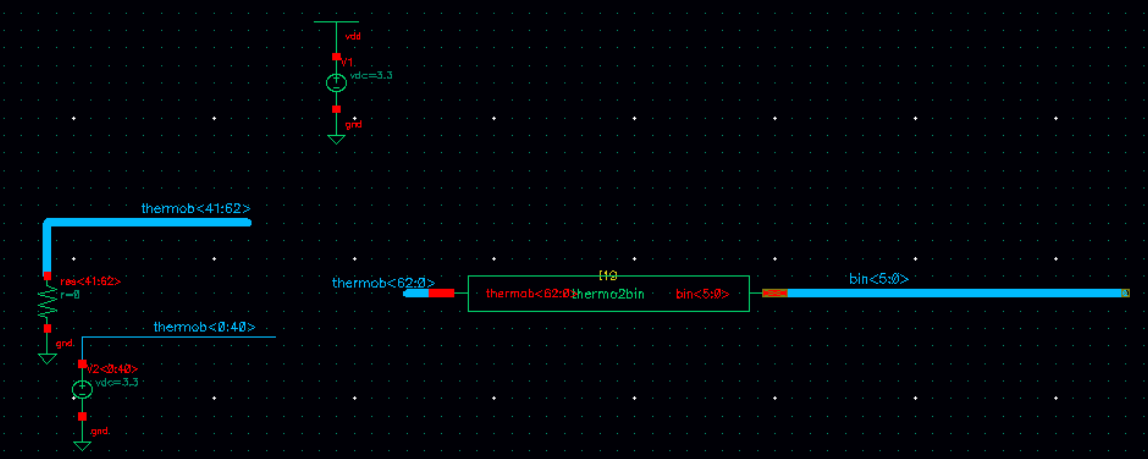
\includegraphics[width=\linewidth]{test_thermo2bin.png}
      \caption{Placement d'un band de test pour le code Verilog apr\`es synth\`ese.}
\end{figure}%

Le bande de test passe les bits de 0 \`a 40 en 1 logique, puis fixe le reste \`a 0. La figure
\ref{fig:simT2B} montre les r\'esultats de la simulation :

\begin{figure}[!htb]
      \centering
      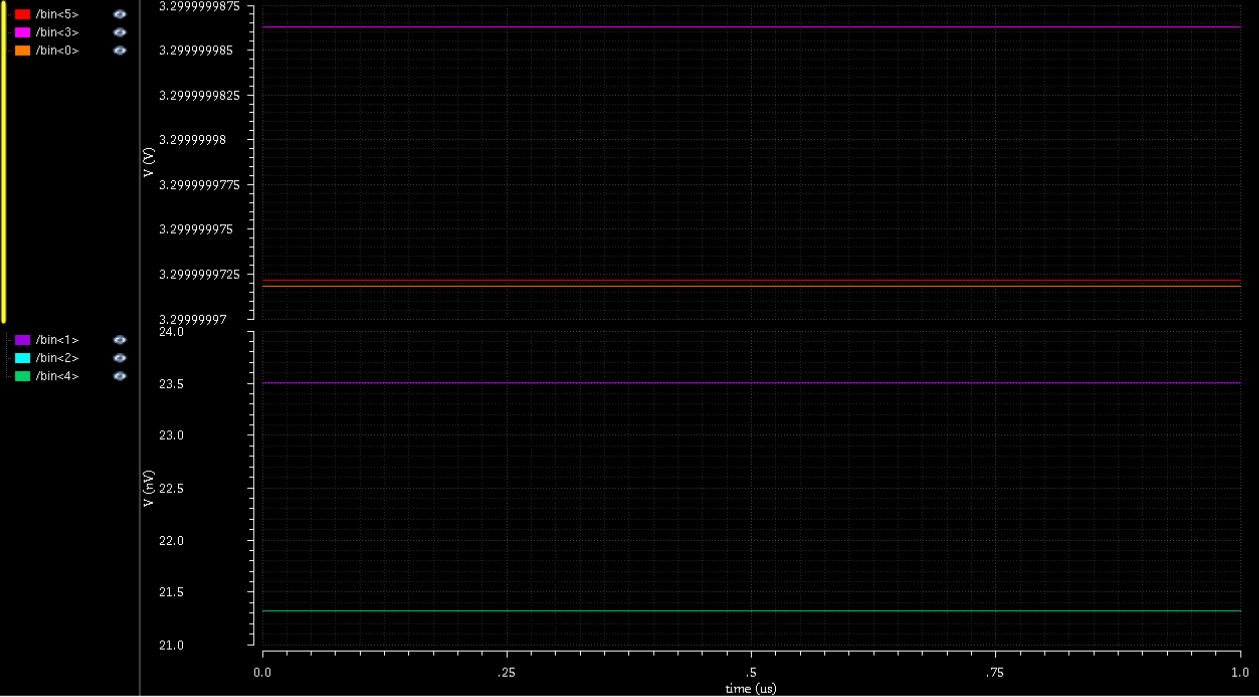
\includegraphics[width=\linewidth]{sim_thermo2bin.png}
      \caption{Simulation d'un code thermom\'etrique pour sa conversion en binaire}
      \label{fig:simT2B}
\end{figure}%

Sachant que le code bin5 est le MSB, bin0 le LSB, on retrouve 101001 ce qui est \'equivalent \`a
l'entr\'ee 41 en code thermom\'etrique.

\clearpage


\section{Sch\'ema Global}
\subsection{Mise en place des \'el\'ements du montage final}
La mise en oeuvre du sch\'ema final se fait par le placement de l'\'echantillonneur bloqueur
ainsi que les 63 comparateurs et le pont de r\'esistances pour la cr\'eation des seuils.

En soi, le sch\'ema est celui de la figure \ref{fig:schemaGlobal} :

\begin{figure}[!htb]
\begin{center}
  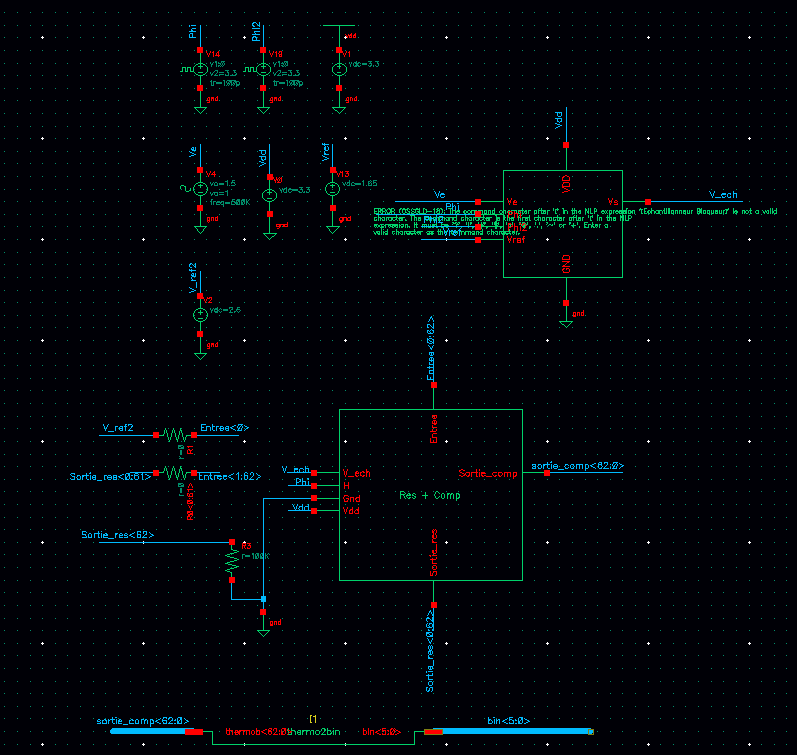
\includegraphics[scale=0.60]{schema_final.png}
  \caption{"Sch\'ema global du CAN-FLASH"}
  \label{fig:schemaGlobal}
\end{center}
\end{figure}

Lors de cette \'etape, nous avons utilis\'e un bloc ``Comparateur + r\'esistance'' que nous avons boucl\'e
sur lui-m\^eme 62 fois dans le but d'\'eviter le sch\'ema \`a rallonge (avec 63 bo\^ites diff\'erentes…).

L'entr\'ee du premier bloc de comparaison (comparateur et seuil gr\^ace \`a la r\'esistance) prend en compte
le signal en sortie de l'\'echantillonneur bloqueur ainsi que le niveau de r\'ef\'erence le plus haut.

Le second \'etage de comparaison a pour entr\'ee la sortie de premier \'etage ainsi que le signal \'echantillonn\'e.
Cet \'etage compare donc le signal \'echantillonn\'e et le seuil num\'ero 2 (deux r\'esistances \'egales en s\'erie).

Le dernier \'etage de comparaison utilise toujours le m\^eme signal \'echantillonn\'e ainsi que le seuil 64 form\'e
de 64 r\'esistances en s\'erie.

\subsection{Simulations}

La simulation globale de cet \'etage est tr\`es int\'eressante. En effet, les courbes pr\'esentent des valeurs de
seuils tr\`es diff\'erentes de celles pressenties par le calcul (niveaux nets cr\'es par des r\'esistances en s\'erie).
En fait, les entr\'ees des comparateurs sont des gros transistors NMOS. Par cons\'equent, leurs capacit\'es d'entr\'ee
sont tr\`es importantes ; une fois reli\'ees \`a des r\'esistances (pont de r\'esistances), des effets de filtrages
apparaissent et d\'egradent les niveaux de seuils.

Les filtres ont en moyenne une fr\'equence de coupure de $\frac{1}{2 \pi R C}$ avec $C  = 90 \phantom{2} fF.$
Pour pallier ce ph\'enom\`ene, nous avons plac\'e un suiveur parfait (vcvs) dans la bo\^ite de comparaison pour
`` purifier '' les niveaux de seuils.

\begin{figure}[!htb]
      \centering
      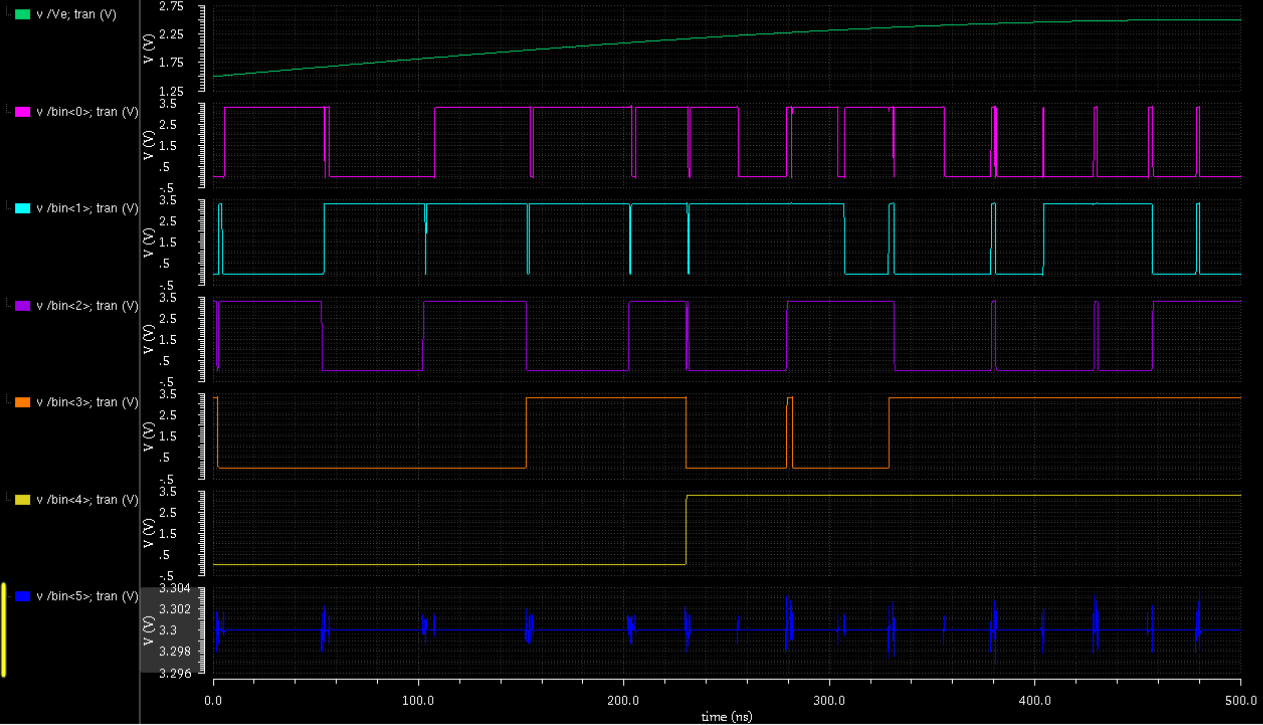
\includegraphics[width=\linewidth]{sim_general.png}
      \caption{Simulation g\'en\'erale du CAN-FLASH pour un quart de signal sinuso\"idal}
      \label{fig:schsimgenerale}
\end{figure}%

Dans la simulation g\'en\'erale, le bin5 repr\'esente le bit MSB en sortie du CAN-FLASH 6-bits, bin0 celui du LSB. On peut voir leur comportement incr\'emental pour un quart d'onde en entr\'ee. 

\clearpage

\section{Layout}
\subsection{Mise en oeuvre}

Le layout constitue l'une des \'etapes n\'ecessaire dans la conception : elle permet de positionner
les diff\'erents \'el\'ements du circuits pour la r\'ealisation des masques.
Vue de la complexit\'e de la r\'ealisation d'un layout complet d'un tel projet, ainsi que les contraintes
du temps impos\'ees, on ne se contente qu'\`a la r\'ealisation d'un simple switch en Layout.

\begin{figure}[!htb]
      \centering
      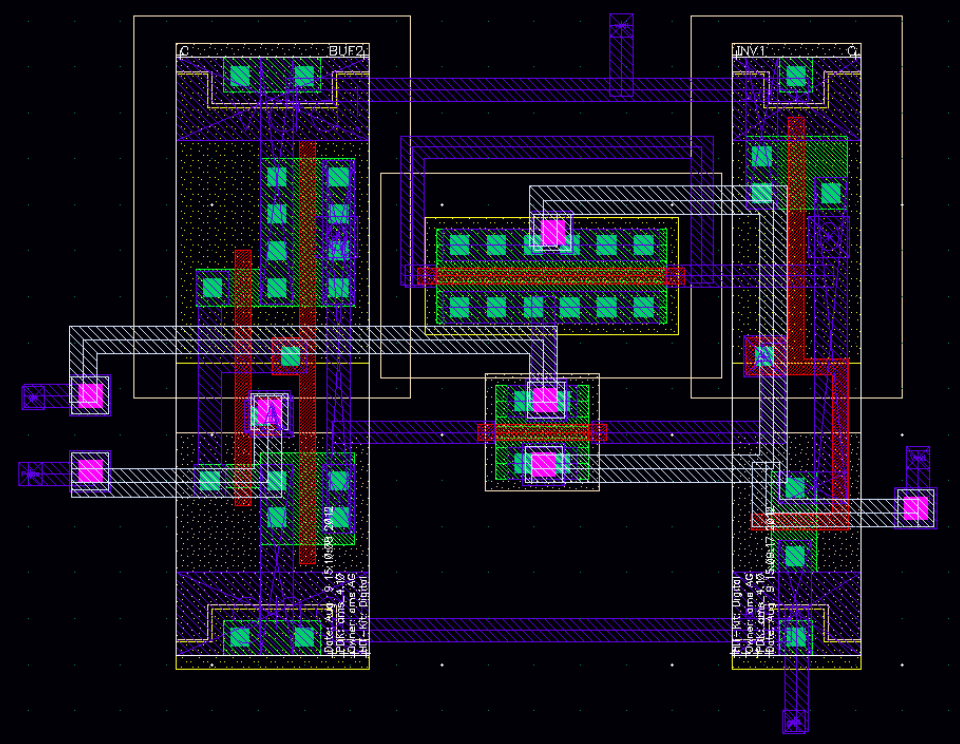
\includegraphics[width=\linewidth]{layout_.png}
      \caption{Mise en place du layout d'un switch}
\end{figure}%

On peut retrouver les \'el\'ements du switch : un buffer et un inverseur pour les signaux d'horloges, ainsi que les deux MOS. On utilise alors deux niveaux de m\'etalisation pour r\'ealiser le sh\'ema \'electrique total, ainsi que des Vias de connection, tous en respectant les r\`egles de dessins du Layout, vis-\`a-vis de l'espacement, et la longueur des liaisons.

Une simulation post-layout peut-\^etre \'etablie pour comparer le fonctionnement obtenu \`a celui du sch\'ema \'electrique.

\clearpage

\section{Am\'eliorations possibles}

Finalement, notre convertisseur fonctionne presque parfaitement : l'\'etage d'\'echantillonneur bloqueur remplit tout \`a fait son r\^ole.
En revanche, certains \'etages de comparaison n'affichent pas toujours la bonne valeur. Th\'eoriquement, si l'\'etage de comparaison n sort
la valeur 1 en code thermom\'etrique, les \'etages $>$ n doivent \'egalement afficher 1 et $<$ n, 0.
Dans nos simulations, il arrive que des \'etages sup\'erieurs soient \`a 0.

Nous soup\c connons les inverseurs et portes NAND de mal interpr\'eter la tension en sortie d'un comparateur et de mal traduire l'information.
Pour contrer ces probl\`emes mineurs (moins d'une comparaison fausse sur 10), il faudrait revoir la partie droite de l'\'etage de comparaison
concernant le latch et la polarisation de sortie. On pourrait par exemple optimiser la puissances des portes logiques ou calculer avec de
plus fins mod\`eles les caract\'eristiques des transistors concern\'e sur le comparateur.

L'\'etage d\'ecodeur de code thermom\'etrique vers binaire fonctionne parfaitement mais est impact\'e par le probl\`eme susmentionn\'e de fausse comparaison.
Il en r\'esulte une erreur d'environ trois valeurs sur 64 ce qui fausse le code binaire final.

\section{Conclusion}

La r\'ealisation d'un CAN Flash 6 bits pr\'esent\'ee dans ce projet fut une bonne exp\'erience dans la mesure o\`u nous sommes d\'esormais conscients
de la complexit\'e \`a r\'ealiser un convertisseur efficace et s\^ur.
Le d\'ebut du projet fut d\'elicat car nous \'etions confront\'es \`a de lourds sch\'emas \'electriques \`a r\'ealiser. Leur optimisation prit du temps et
passa par de nombreux calculs th\'eoriques vus en cours de convertisseurs ou d'\'electronique analogique.
Ce projet fut \'egalement l'occasion de v\'eritablement prendre en main le logiciel Virtuoso de Cadence \`a travers les outils de simulation,
 de variables ajust\'ees, de sources de courant ou tension parfaites. Nous maîtrisons d\'esormais ce logiciel et sommes aptes \`a l'utiliser \`a
 des fins de recherche ou dans l'industrie.

Nous sommes ravis d'avoir pu r\'efl\'echir par nous-m\^eme et mobiliser nos connaissances acquises dans plusieurs cours cette ann\'ee au service
de ce projet. Il a eu un r\'eel impact sur notre maîtrise de Cadence et sur le d\'eroulement de la phase de conception d'un circuit \'electronique,
en l'occurrence d'un comparateur Flash.

Nous remercions les professeurs encadrants de nous avoir transmis leurs connaissances et astuces dans le domaine, nous les utiliserons
\`a bon escients \`a l'avenir.

\clearpage

\section{Fiche descriptive des caract\'eristiques}

\clearpage

\section{Annexes}
\subsection{Calcul th\'eorique complet de l'amplificateur}\label{Annexe1}

\textbf{Cahier des charges :} 
\begin{itemize}\itemsep -4pt
\item $V_{EMC} \in [0.5; 2.5V]$ en entr\'ee.
\item gain en basse fr\'equence $G(0) \in [300;400]$
\item $C_{S} = 6 pf$
\item Dyanmique en sortie : $V_{S} \in [0.5; 3.5V]$ 
\end{itemize}

La figure \ref{fig:schemaAOP-OTA} repr\'esente l'amplificateur OTA \`a deux \'etages pris
en consid\'eration, qui \'etait \'etudi\'e en cours de conception des circuits int\'egr\'es analogique\cite{TD4-AOP}.
On reprend ce circuit en l'adoptant \`a nos besoins, selon le cahier de charge bien d\'efini.

\begin{figure}[!htb]
      \centering
      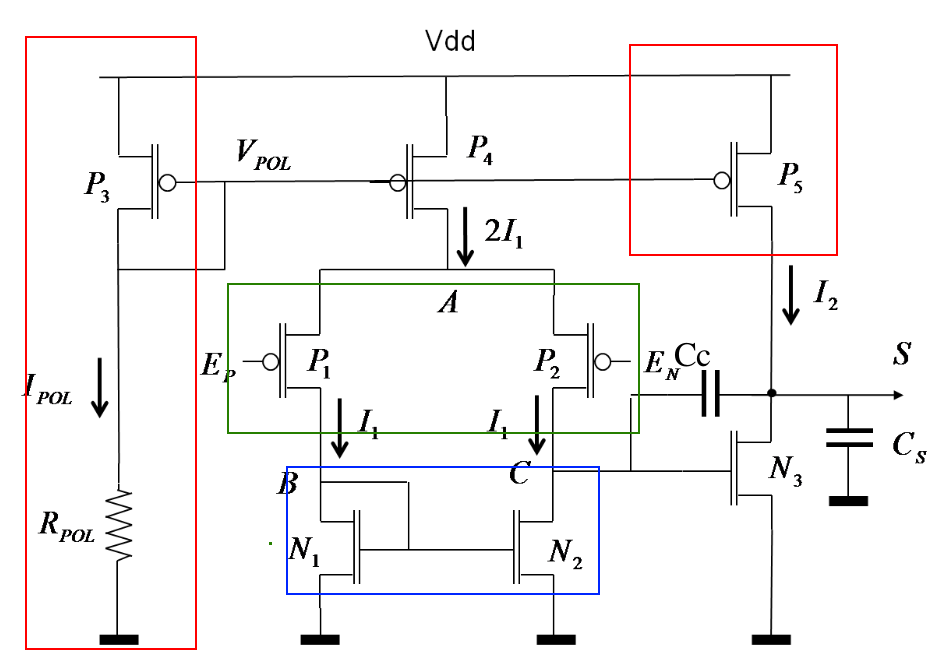
\includegraphics[width=0.6\linewidth]{schema_composition_AOP_2_etages.png}
      \caption{Sch\'ema th\'eorique de l'amplificateur avec les diff\'erentes fonctionnalit\'es des \'etages}
      \label{fig:schemaAOP-OTA}
\end{figure}%

Foncionnalit\'e des \'etages :
\begin{itemize} \itemsep -2pt
\item[-] Bloc Vert : Transistors $P_{1,2}$ constitue la paire diff\'erentielle.
\item[-] Bloc Bleu : Couple NMOS $N_{1,2}$ fonctionnant en mirroir de courant (charge active).
\item[-] Bloc Rouge : Couple PMOS $P_{3,5}$ ainsi qu'une r\'esistance, fonctionnant comme mirroir de courant
  pour injecter un courant $I_{POL}$ dans $N_{3}$
\end{itemize}

\textbf{Calcul Th\'eorique}\\
On commence par calculer les valeurs de $V_{pol}, I_{pol}$ (tension et courant de polarisation)
ainsi que les valeurs aux noeuds A, B, C de fa\c con qu'on se limite aux cahier de charge ainsi d\'efini.

\textbf{On fixe la polarisation des PMOS $P_{1,2}$ \`a $0.2 V$}\\
On cherche alors $V_{pol}$ de sorte qu'elle v\'erifie le maximum de la dynamique en entr\'ee et respecte bien
celle en sortie :

\clearpage

Au point A :
$V_{A_{max}}$ qui correspond \`a $V_{E_{max}}$ (on consid\`ere aussi l'effet substrat sur $P_1$ et $P_2$)
\[
\bigg( V_{sg} - | V_{tp} | \bigg)_{P_{1,2}} = V_{A_{max}} - V_{E_{max}} - |V_{tp}| = V_{A_{max}} - V_{E_{max}} -
\Big( | V_{tp_{0}} | + 0.2(V_{dd} - V_{A_{max}})\Big)
\]
\[
1.2V_{A_{max}} - V_{E_{max}} - | V_{tp_{0}} | - 0.2 V_{dd} = 0.2
\]
\[
V_{A_{max}} = \frac{1.6 + V_{E_{max}}}{1.2}
\]
Pour $V_{E_{max}} = 2.5$, on obtient $V_{A_{max}} = 3.41 V$

Sachant que la tension $V_{A_{max}}$ doit satisfaire la limite de la zone active du PMOS $P_4$ pour qu'il
fonctionne, on :
\[
\Big(V_{sd}\Big)_{P_{4}} = \Big(V_{sg} - | V_{tp_{0}} | \Big)_{P_4} 
\]
ce qui implique que : 
\[
V_{dd} - V_{A_{max}} = V_{dd} - V_{pol} - |V_{tp_0}|
\]
\[
V_{A_{max}} = V_{pol} + |V_{tp_0}|
\]
\[
V_{pol} = 3.41 - 0.73 = 2.68 V
\]

Cette valeur satisfait la condition sur $V_{E_{max}}$.

Pour la dynamique en sortie, on a trouve que la dyamique de $V_S$ est fix\'ee par la LZA de $P_5$ :
\[
V_{dd} - V_{S_{max}} = V_{dd} - V_{pol} - |V_{tp_0}|
\]

On retrouve que :
\[
V_{S_{max}} = V_{pol} + 0.73 = 2.68+0.73 = 3.41 V \leq 3.5 V 
\]
$V_{pol}$ respecte la dynamique de sortie sur $V_{S_{max}}$. Par rapport \`a la condition minimale de la
dynamique en sortie, on doit retrouver $V_C = V_B$ au points B et C.

On doit avoir $V_{S_{min}} = V_C - V_{tn_0}$ pour que le NMOS $N_3$ reste en LZA.
Soit :
\[
V_C = V_{S_{min}} + 0.57 = 1.07 V = V_B
\]

Il nous reste de v\'erifier que la limite inf\'erieure de la dynamique en $V_e$ est toujours respect\'ee,
celci d\'ependante de la tension $V_{A_{min}}$ :

\[
\bigg( V_{sg} - | V_{tp} | \bigg)_{P_{1,2}} = V_{A_{min}} - V_{E_{min}} - |V_{tp}| = V_{A_{min}} - V_{E_{min}} -
\Big( | V_{tp_{0}} | + 0.2(V_{dd} - V_{A_{min}})\Big) = 0.2V
\]

\[
V_{A_{min}} = \frac{1.6 + V_{E_{min}}}{1.2} = 1.75 V
\]

\[
\bigg( V_{sg} - | V_{tp} | \bigg)_{P_{1,2}} = 0.2V \leq V_{A_{min}} - V_C = 1.75 - 1.07 = 0.68 V
\]

On trouve bien qu'elle respecte la valeur minimale.

\clearpage

Avec la valeur des tensions $V_{A}, V_{B}, V_{C}, V_{pol}$, on peut remonter aux valeurs des courants dans
les diff\'erentes \'etages de l'amplificateur.

\textbf{Calcul de $I_1, I_2, I_{pol}$ :} \\
Pour $I_1 = \frac{I_{pol}}{2} = \frac{I_{2}}{10}$ et $P = 2 mW$, on retrouve :
\[
2I_1 + I_2 = 0.6 mA
\]
$I_{pol}$ n'est pas pris en consid\'eration sachant qu'il peut \^etre commun aux autres cellules.

On retrouve : $ I_2 = 500 \mu A, I_1 = 50 \mu A, I_{pol} = 100 \mu A$.

La r\'esistance de polarisation peut-\^etre facilement retrouver : $R_{pol} = \frac{V_{pol}}{I_{pol}}$
avec $V_{pol} = 2.68 V$, $ R_{pol} = 26.9 k \Omega$.

\textbf{Dimensionnements des transistors} :\\
Avec la d\'etermination des courants et tensions de polarisation, on peut retrouver les
rapport $\Big( \frac{W}{L} \Big)$ des diff\'erents transistors :

Rappelons que :
\[
\bigg( \frac{W}{L} \bigg)_{P} = \frac{I_{sd}}{K_p \big( V_{sg} - |V_{tp}| \big)^{2} }
\phantom{3} et \phantom{3}
\bigg( \frac{W}{L} \bigg)_{N} = \frac{I_{ds}}{K_N \big( V_{gs} - |V_{tn}| \big)^{2} } 
\]
\[
\bigg( \frac{W}{L} \bigg)_{P_{1,2}} = 50
\phantom{3}
;
\phantom{3}
\bigg( \frac{W}{L} \bigg)_{P_{4}} = 277
\phantom{3}
;
\phantom{3}
\bigg( \frac{W}{L} \bigg)_{N_{1,2}} = 10
\]
Par rapport \`a $N_3$ et $N_2$ (sachant que $V_B = V_C$) :
\[
\bigg( \frac{W}{L} \bigg)_{N_{3}} = \frac{I_2}{I_1} \bigg( \frac{W}{L} \bigg)_{N_{2}}  = 100  
\]

Pour $P_5$, la condition sur le mirroir de courant ne ram\`ene \`a :
\[
\bigg( \frac{W}{L} \bigg)_{P_{5}} = \frac{I_2}{2 I_1} \bigg( \frac{W}{L} \bigg)_{P_{4}} = 220
\]

Si on fixe $L_N = 0.35 \mu m$ et $L_P = 0.7 \mu m$ pour les PMOS respectivement, on peut calculer les
valeurs de $W$ de chaque TMOS :
\[
W_{N_1,N_2} = 3.5 \mu m, W_{N_3} = 35 \mu m, W_{P_1, P_2} = 35 \mu m, W_{P_4} = 193.9 \mu m, W_{P_5} = 969 \mu m
\]

On peut toujours v\'erifier que le gain qu'on cherche respecte bien $G(0)$ d\'efini en cahier de charge
pour une r\'esolution de 6-bits.

Le montage est form\'e de 2 \'etages:
\[
G_1 = - g_m (P_2).r_{ds}(P_2)//r_{ds}(N_2) = -g_m(P_2).\frac{r_{ds}(N_2)}{2}
\]
gain du premier,
\[
G_2 = - g_m (N_3).r_{ds}(N_3)//r_{ds}(P_5) = -g_m(N_3).\frac{r_{ds}(N_3)}{2}
\]
pour le deuxi\`eme.

Sachant que :
\[
g_m(P_2) = \frac{2I_1}{V_{sg} - | V_{tp} | } = 0.5  mA/V
\phantom{3}
;
\phantom{3}
g_m(N_3) = \frac{2 I_2}{V_{gs} - V_{tn}} = 0.598 mA/V
\phantom{3}
;
\phantom{3}
\]

\[
\frac{r_{ds}(N_3)}{2} = \frac{L_{N_{3}}}{2.k_{en}.I_{2}} = 11.7 K\Omega
\phantom{3}
;
\phantom{3}
\frac{r_{ds}{P_2}}{2} = \frac{L_{P_{2}}}{2.k_{ep}.I_{1}} = 117 k\Omega
\]

On retrouve $G_0 = G_1 \times G_2 = 400, (G_0)_{db} = 52 db > 49.5 db$, ce qui correspond bien \`a la
au cahier des charges.


\clearpage

\addcontentsline{toc}{section}{R\'ef\'erences}

\begin{thebibliography}{9}
\bibitem{Projets-Analog}
\textit{Projets de conception en Micro\'electronique analogique}\\
\texttt{Laurant Aubard, Fatah Rarbi, Daniel Zahini, Florent Cilici}\\
\texttt{Institut Polytechnique de Grenoble - Phelma}

\bibitem{Razavi}
\textit{Design of Analog CMOS Integrated Circuits}
\\\texttt{Behzad Razavi, McGraw-Hill Higher Education.}

\bibitem{Razavi-Data-Conversion}
  \textit{AnalogtoDigital Converter Architectures}
\textit{in Principles of Data Conversion System Design}\\
\texttt{Behzad Razavi, Wiley-IEEE Press, 1995, pp.96-152}.\\
\textbf{doi: 10.1109/9780470545638.ch6}

\bibitem{Thermometer}
\textit{Verilog HDL model based thermometer-to-binary encoder with bubble error correction}\\
\texttt{Zbigniew Jaworski, Warsaw University of Technology}\\
\textit{Conference: 2016 MIXDES - 23rd International Conference "Mixed Design of Integrated Circuits and Systems"}\\
\textbf{doi: 10.1109/MIXDES.2016.7529741}

\bibitem{cours-conversion}
\textit{La conversion analogique/num\'erique : Principe et architecture int\'egr\'es}\\
\texttt{S.Bourdel, Institut Polytechnique de Grenoble - Phelma}

\bibitem{TD4-AOP}
\textit{Etude d'un amplificateur CMOS \`a deux \'etages,}\\
\textit{Conception des circuits int\'egr\'es analogiques}\\
\texttt{Laurent Aubard, Institut Polytechnique de Grenoble - Phelma}

\end{thebibliography}


\end{document}
